
\documentclass{beamer}
\usetheme{metropolis} % Use metropolis theme





\title{ECON 3818: Introduction to Statistics with Computer Applications}
%\subtitle
\date{\today}
\author{Kyle Butts}



\definecolor{blue}{RGB}{0,114,178}

\definecolor{red}{HTML}{EB0E09}
\definecolor{yellow}{RGB}{240,228,66}
\definecolor{green}{RGB}{0,158,115}
\definecolor{maroon}{HTML}{AF3335}
\definecolor{purple}{HTML}{7E90B8}


\definecolor{mybackground}{HTML}{ECECEC}
\setbeamercolor{background canvas}{bg= mybackground}

\definecolor{buff-gold}{HTML}{CFB87C}
\definecolor{buff-grey}{HTML}{565A5C}
\definecolor{buff-lightgrey}{HTML}{A2A4A3}
\definecolor{buff-black}{HTML}{000000}

\setbeamercolor{alerted text}{fg=buff-gold!80!black}
\setbeamercolor{frametitle}{bg=buff-black}
\setbeamercolor{title}{fg=buff-grey}
\setbeamercolor{button}{bg=buff-gold}

% Allow to remove indent w/ \begin{itemize}[leftmargin= *]
\usepackage{enumitem}
\setlist[itemize]{label= \textbullet}

% \usepackage[libertine]{newtxmath}
\usepackage{longtable}
\usepackage{booktabs}
\usepackage{enumitem}







\begin{document}

% Title Page ---------------------------------------
\maketitle




% Chapter 3 ----------------------------------------
\section{Chapter 3: The Normal Distribution}

\begin{frame}{Normal Distribution}
    
	Normal curve is symmetric about the mean and bell-shaped
	\begin{center}
		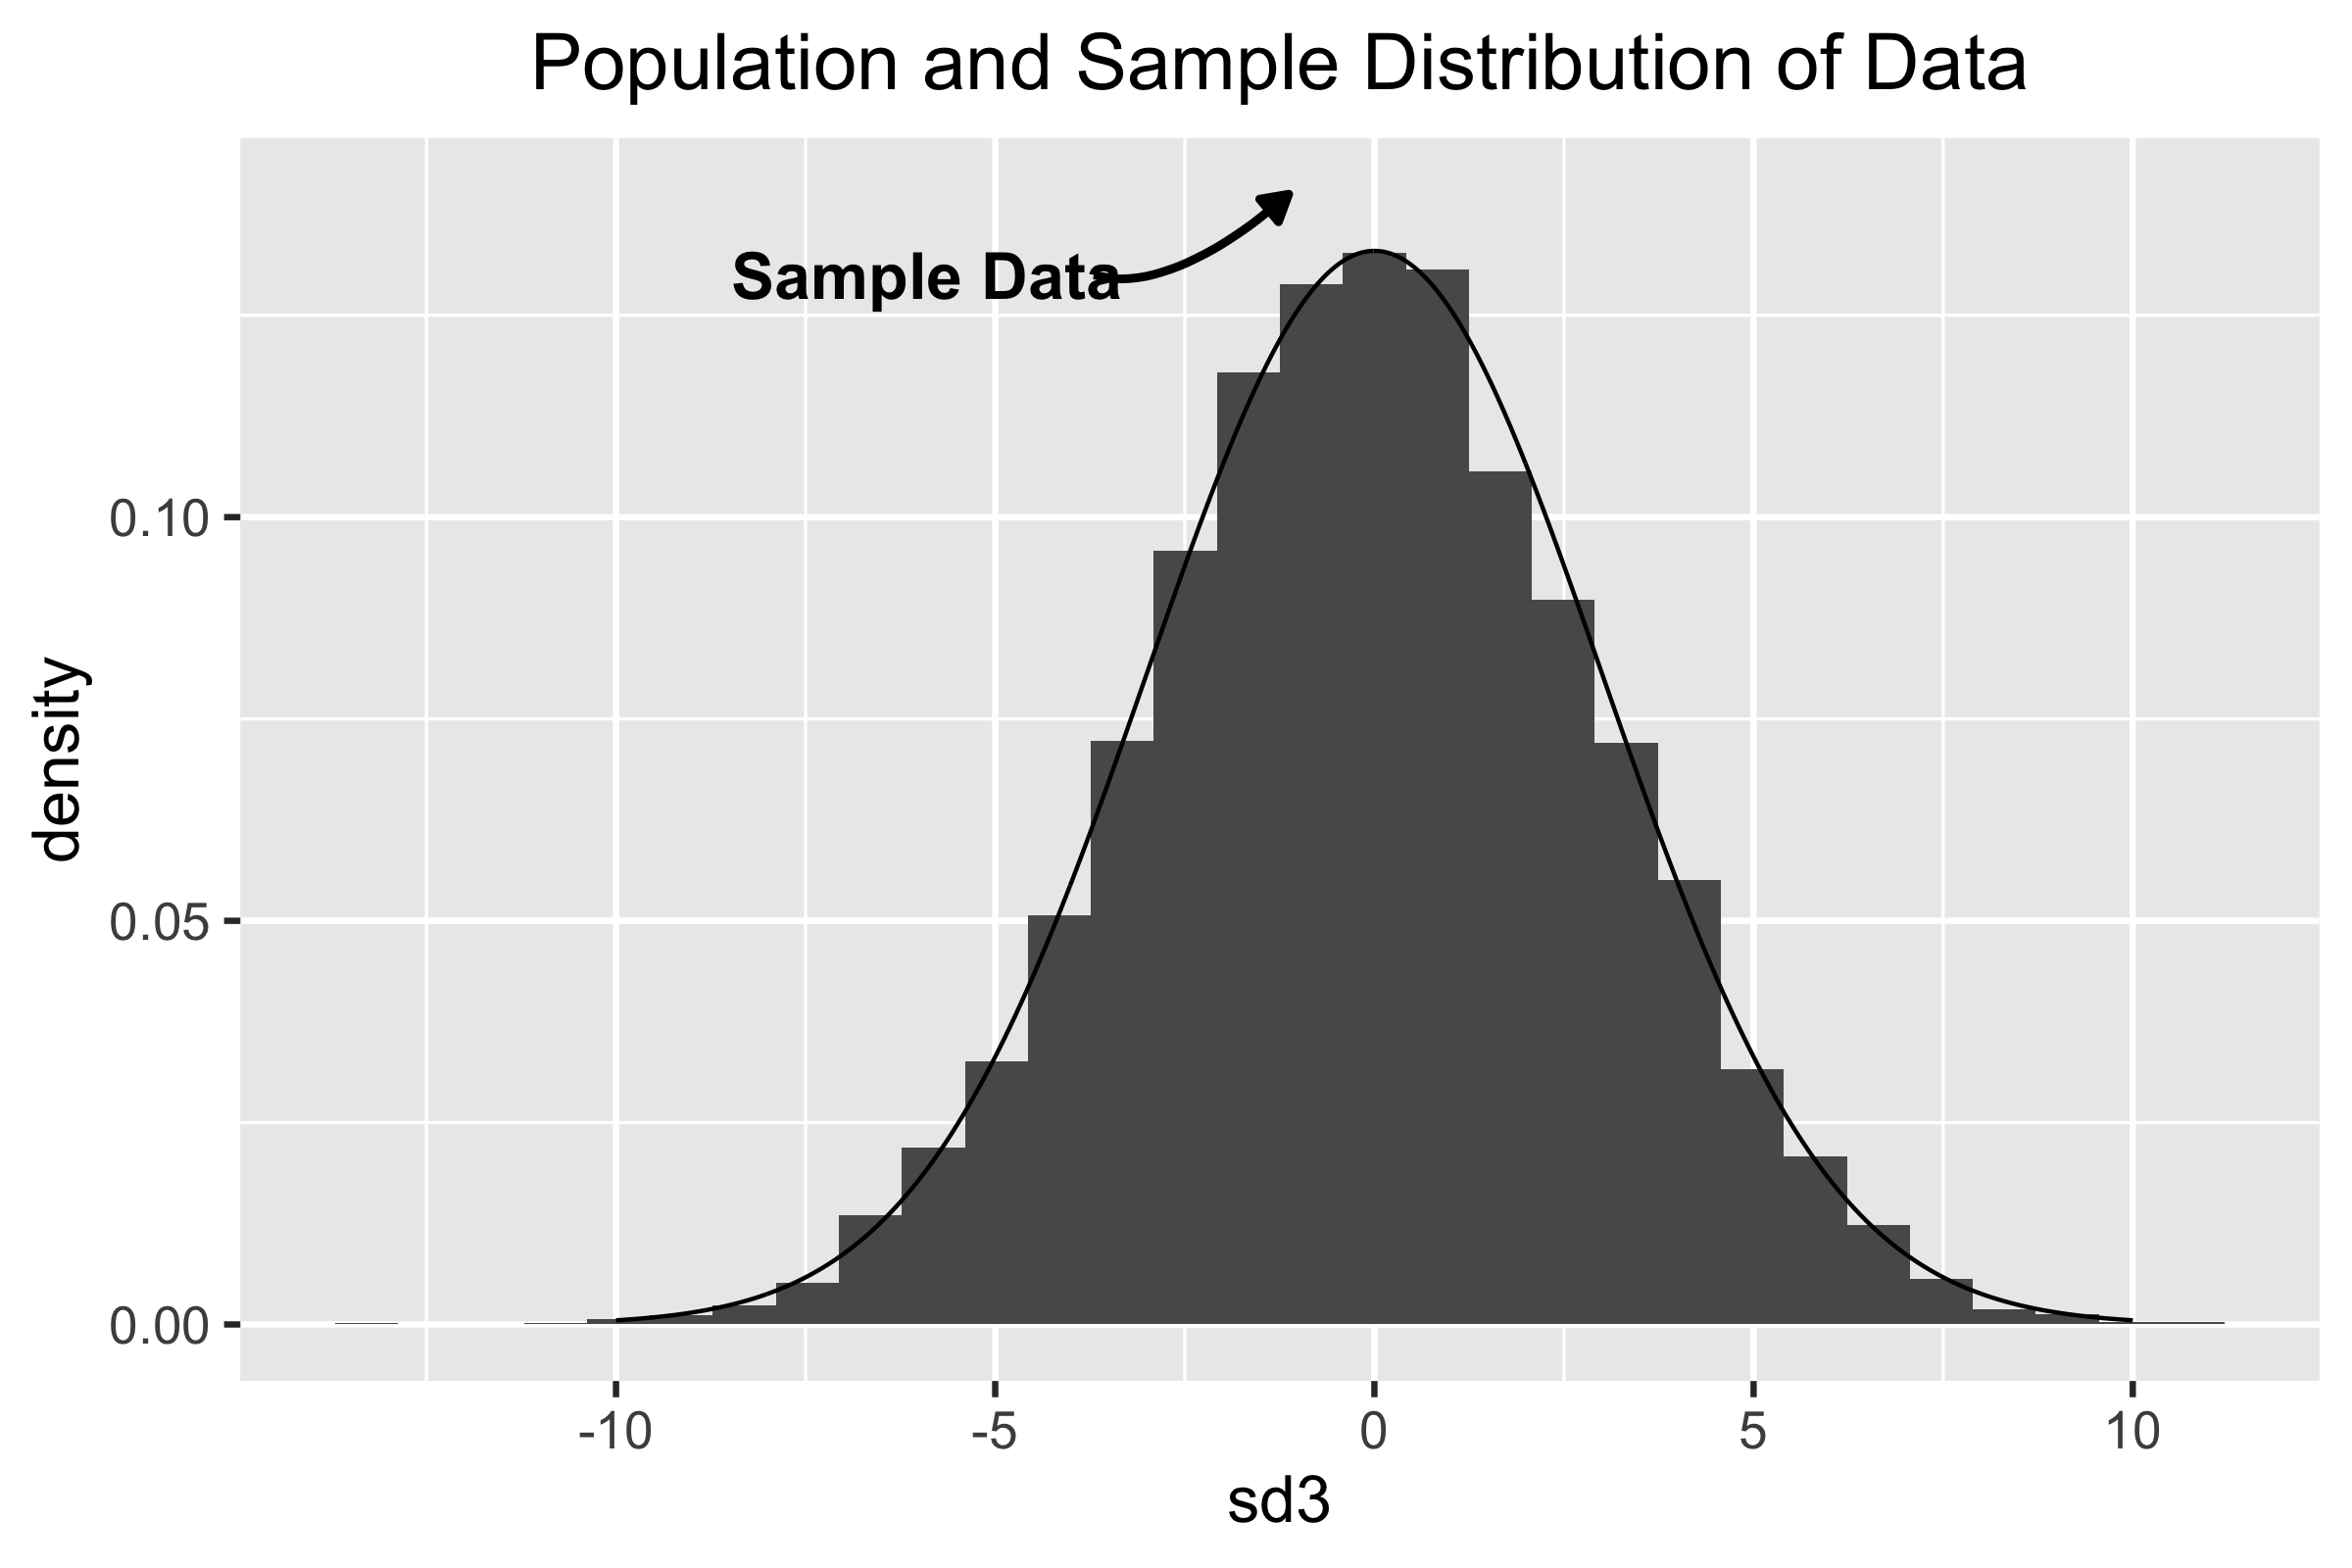
\includegraphics[width=0.6\textwidth]{normdistnsamplehist.png}
    \end{center}
    
	Lots of data naturally follow this distribution
	\begin{itemize}
		\item heights of people, blood pressure, grades on a test
		\item https://www.youtube.com/watch?v=EvHiee7gs9Y
	\end{itemize}
\end{frame}


\begin{frame}{Probability with Histograms: Sample Probability}
    
	\begin{center}
        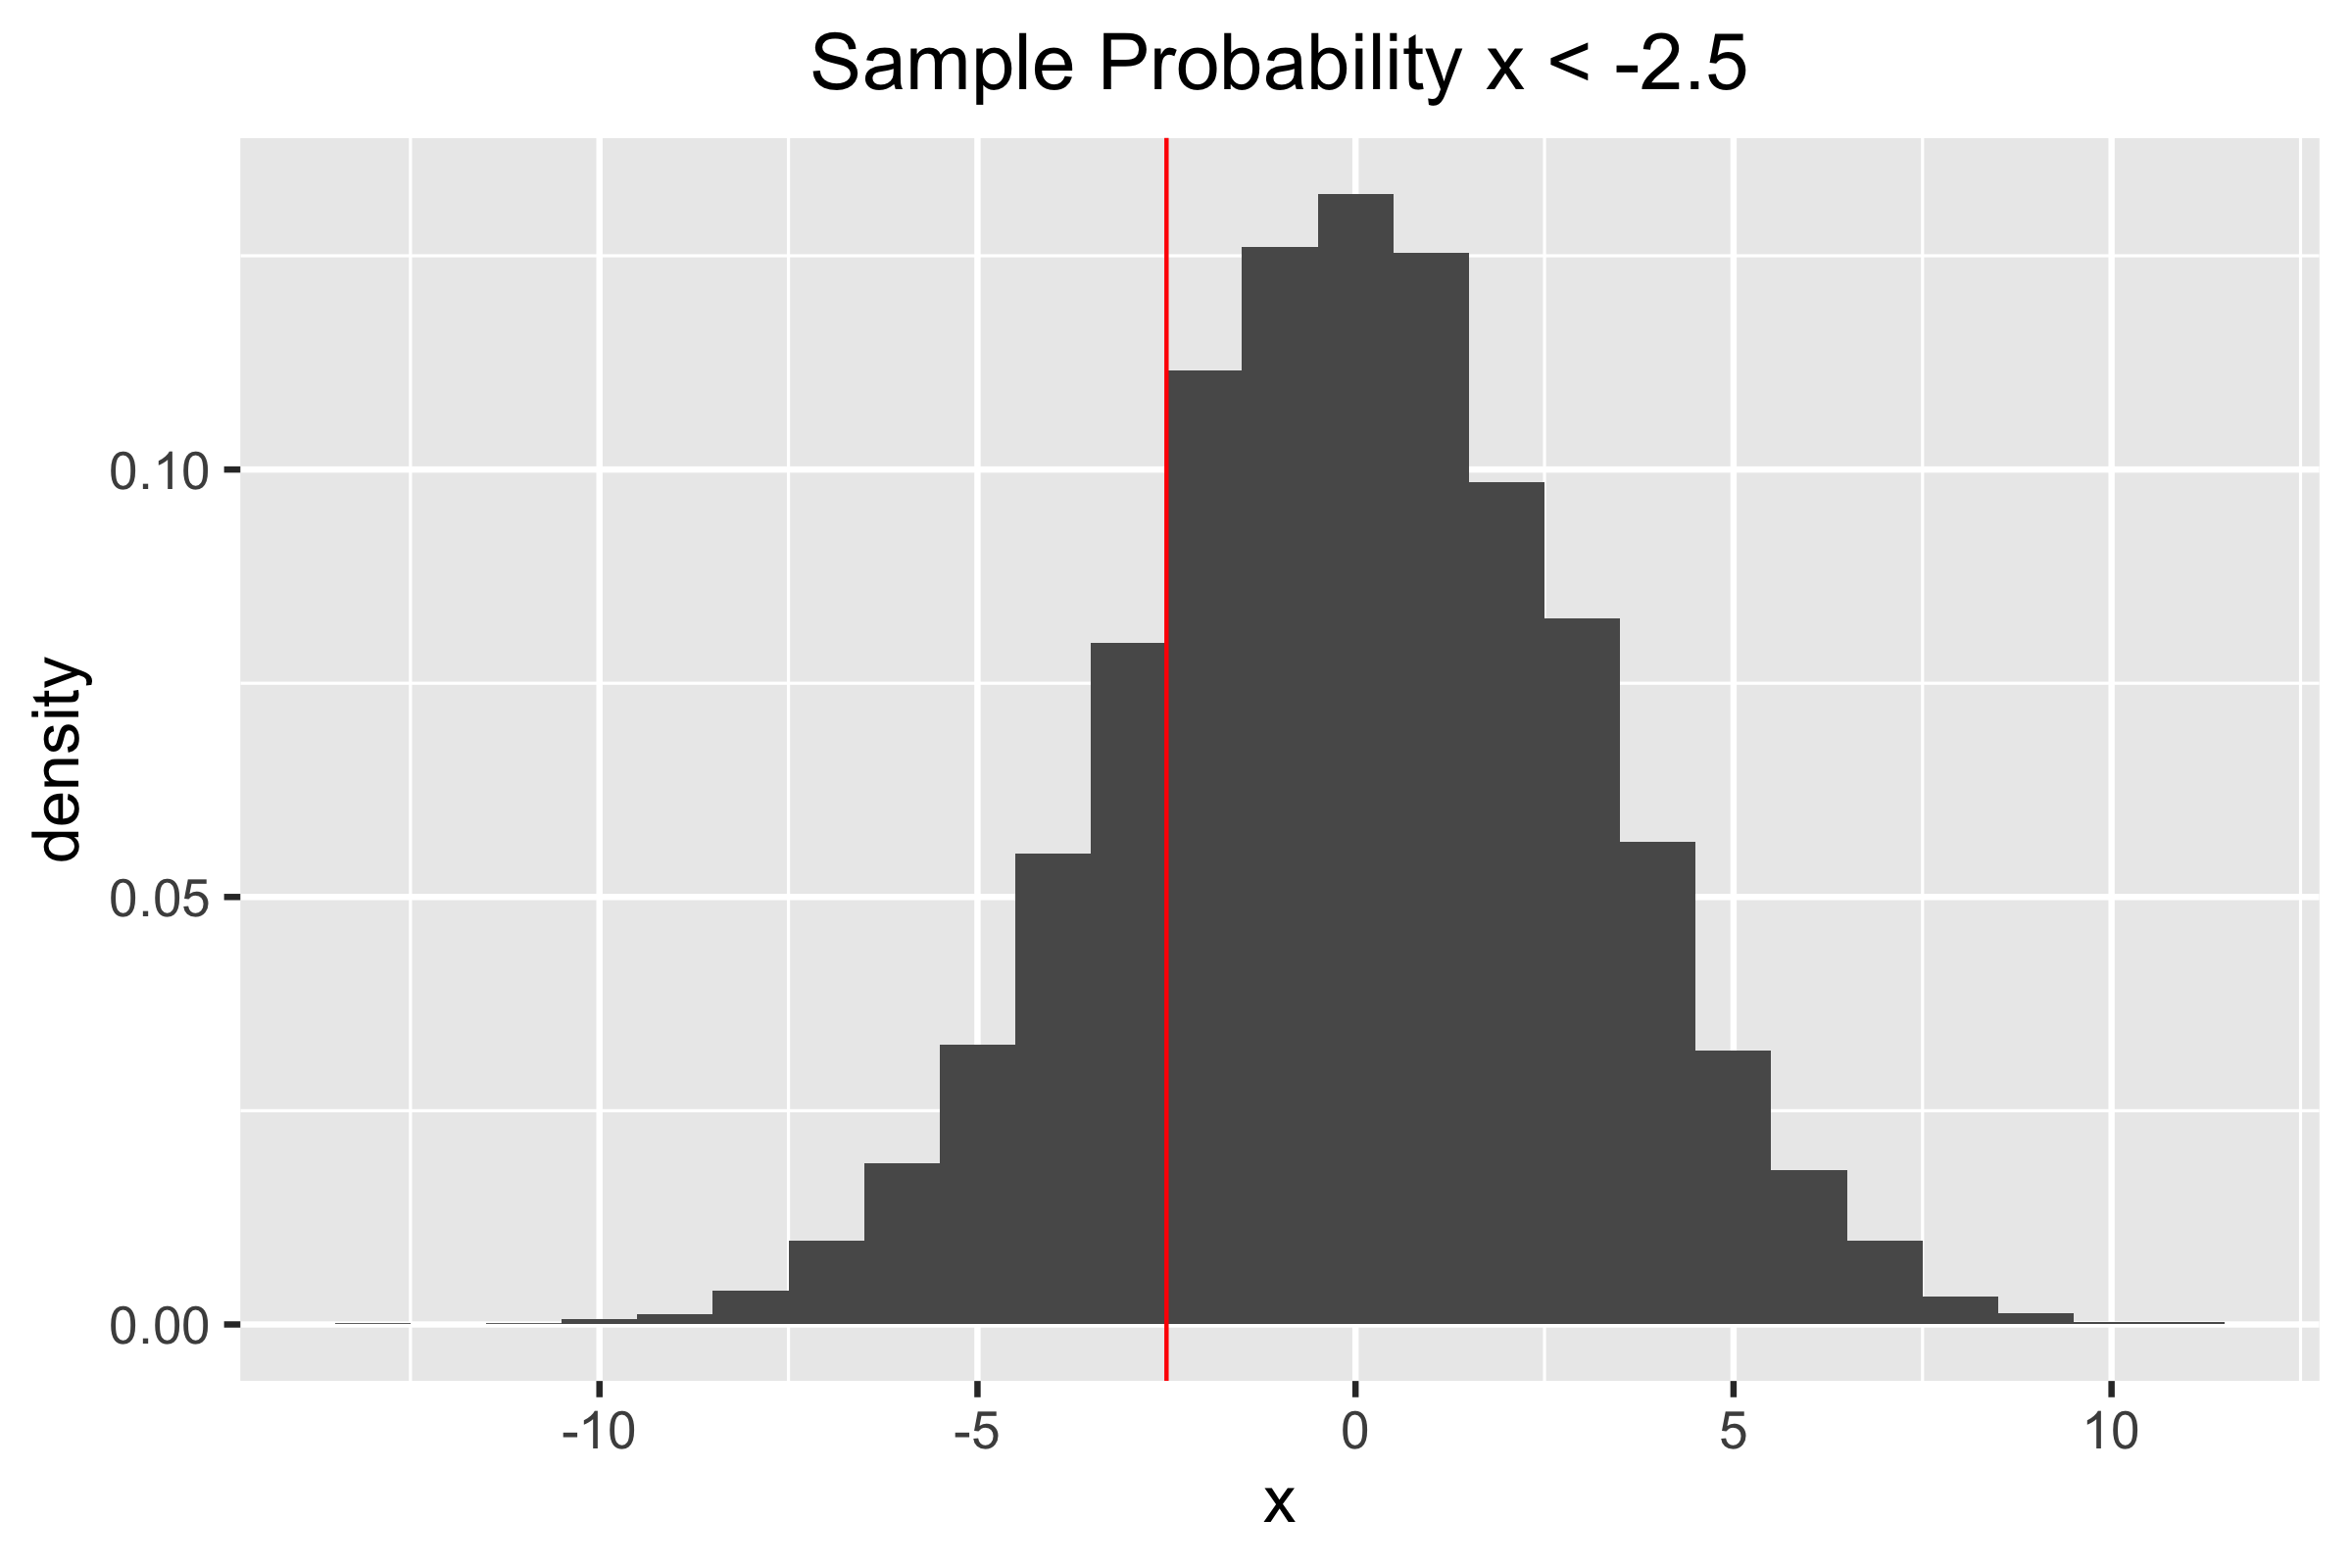
\includegraphics[width=0.6\textwidth]{samp_prob.png}
    \end{center}

    \begin{itemize}
        \item What's the probability that the x value is less than -2.5 in our sample?
    \end{itemize}
\end{frame}

\begin{frame}{Probability with Densities: Population Probability}
    
	\begin{center}
        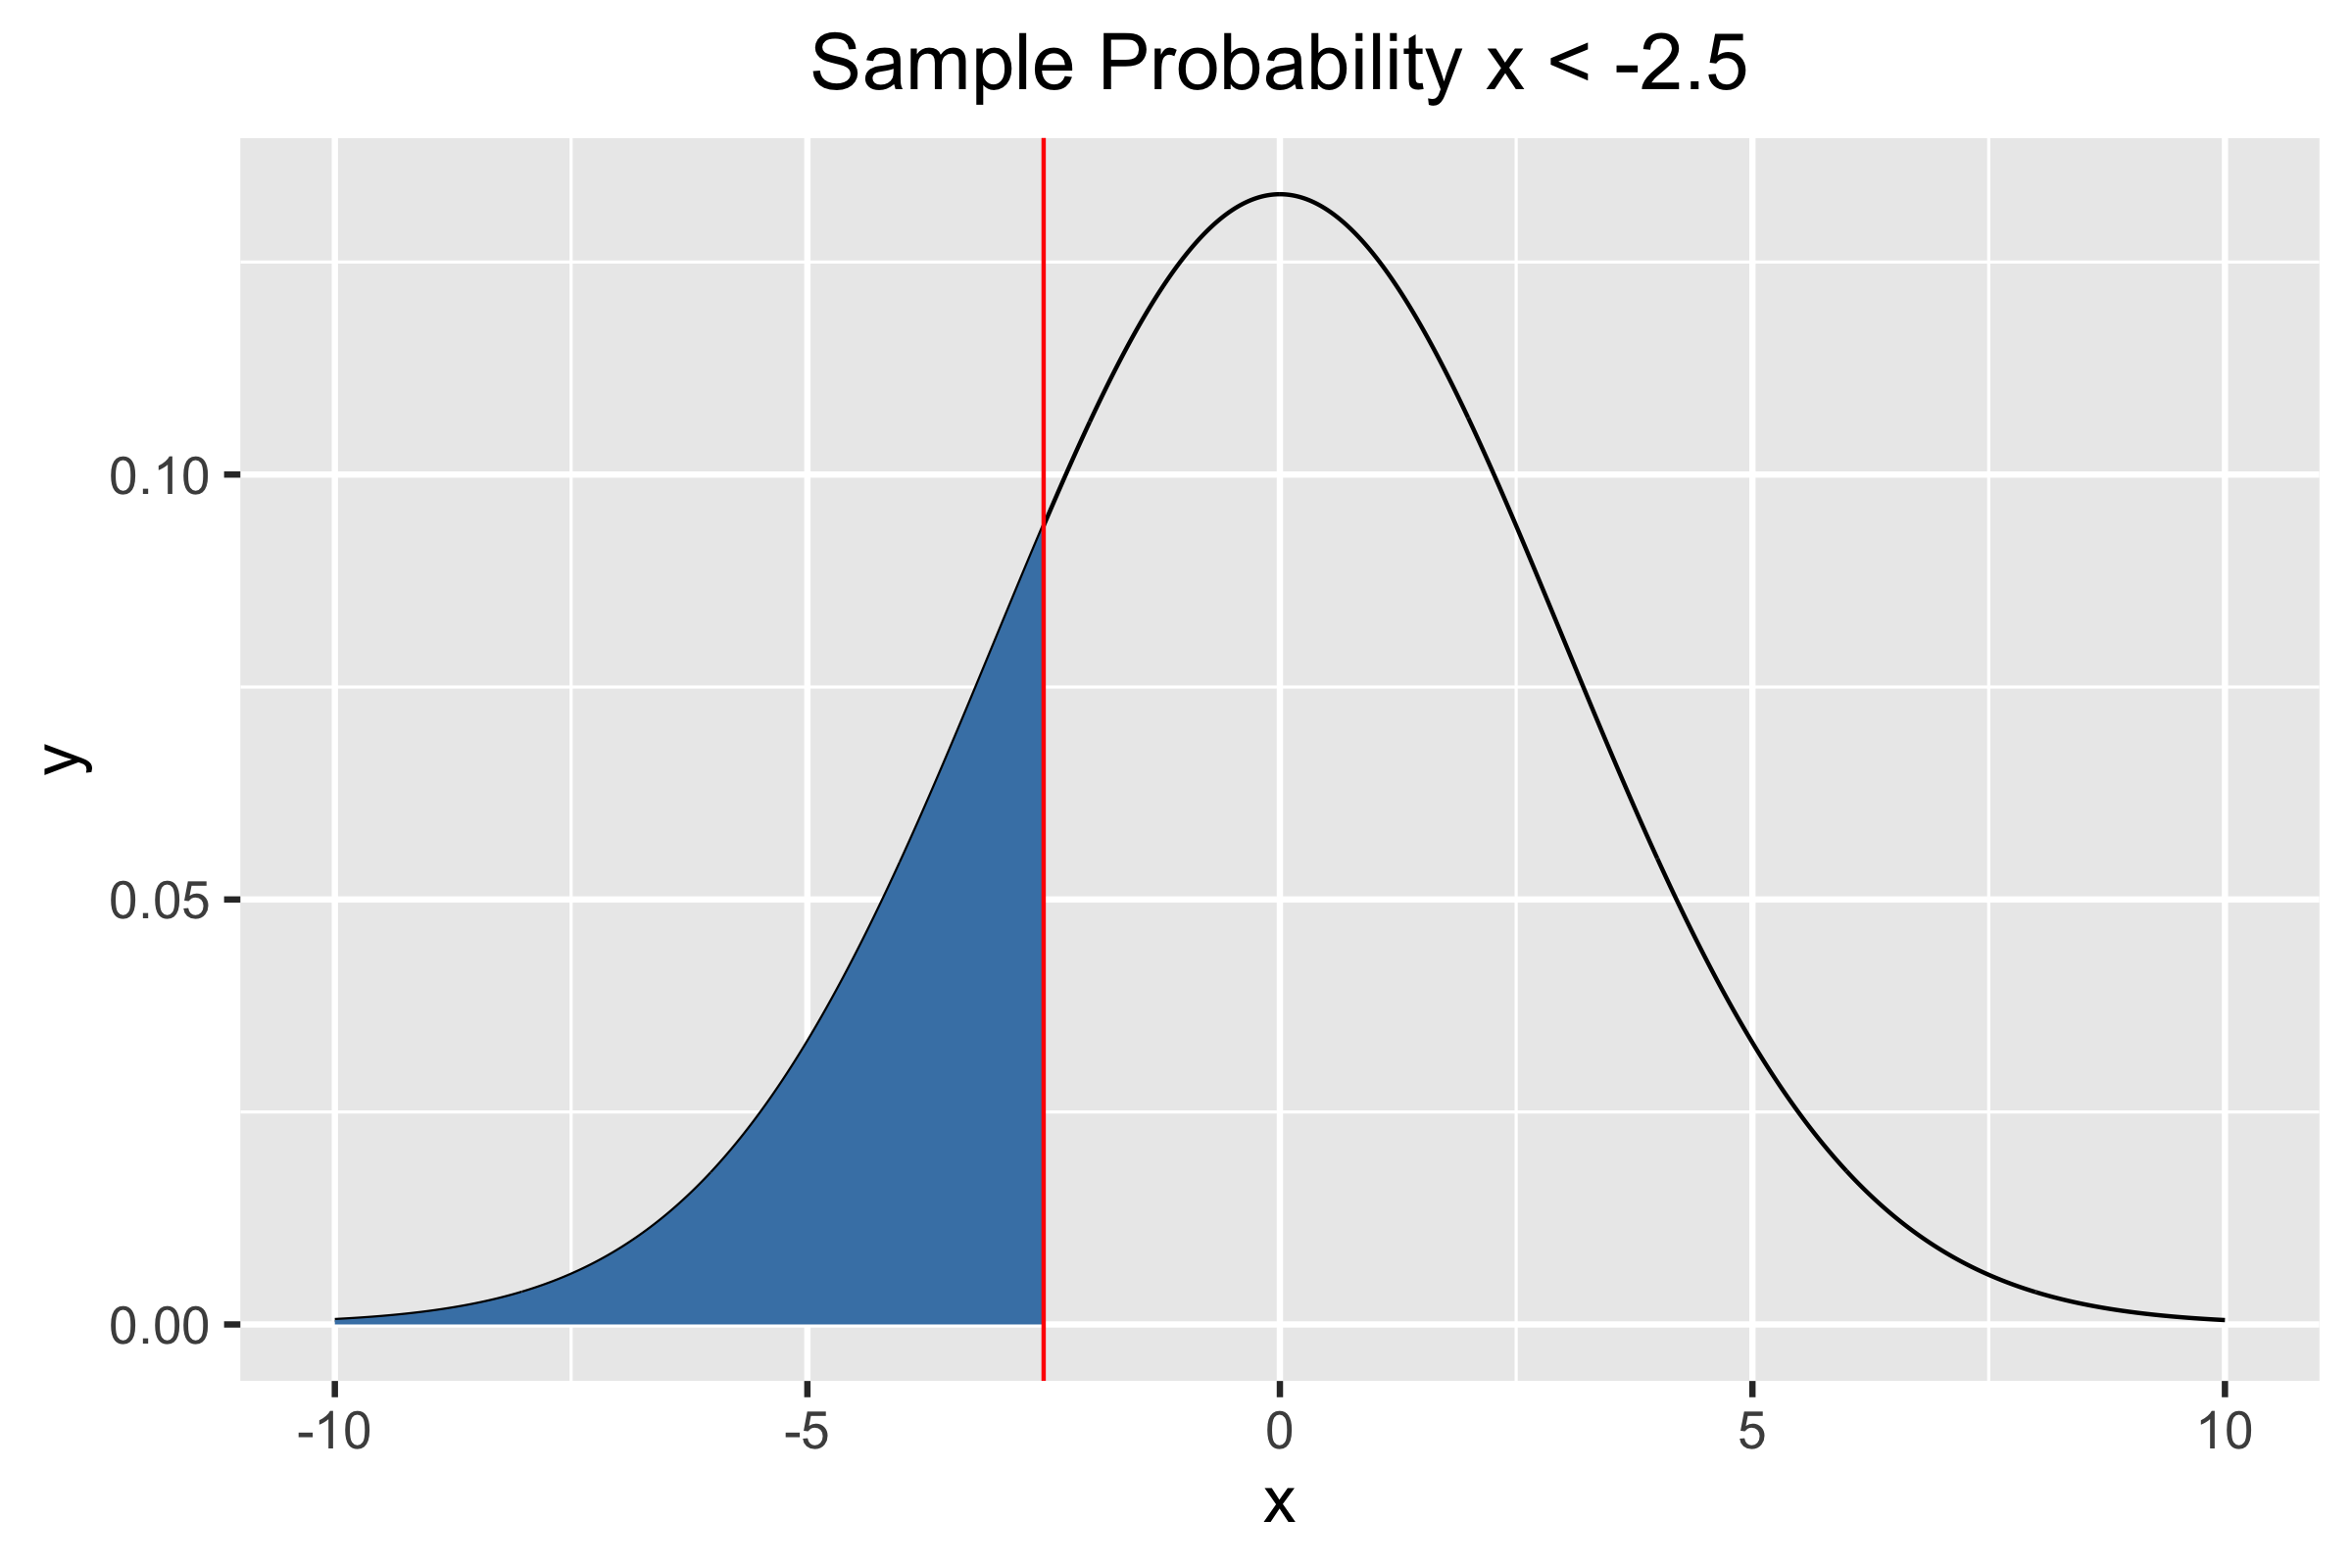
\includegraphics[width=0.6\textwidth]{pop_prob.png}
    \end{center}

    \begin{itemize}
        \item What's the probability that the x value is less than -2.5 in our population distribution?
    \end{itemize}
\end{frame}



\begin{frame}{Parameters of Normal Distribution}
	
	Normal distribution is described by two parameters-- its mean $\mu$ and variance $\sigma^2$
	\begin{itemize}
		\item The mean is located at the center of the symmetric curve
		      \begin{itemize}
		      	\item It is the same as the median 
		      	\item Changing $\mu$ (without changing $\sigma^2$), moves the curve along the horizontal axis
		      \end{itemize}
		\item The variance describes the variability of the curve
		      \begin{itemize}
		      	\item Higher variance means a flatter and wider distribution
		      \end{itemize}
	\end{itemize}
	
\end{frame}

\begin{frame}{Different Variances}
    \begin{center}
        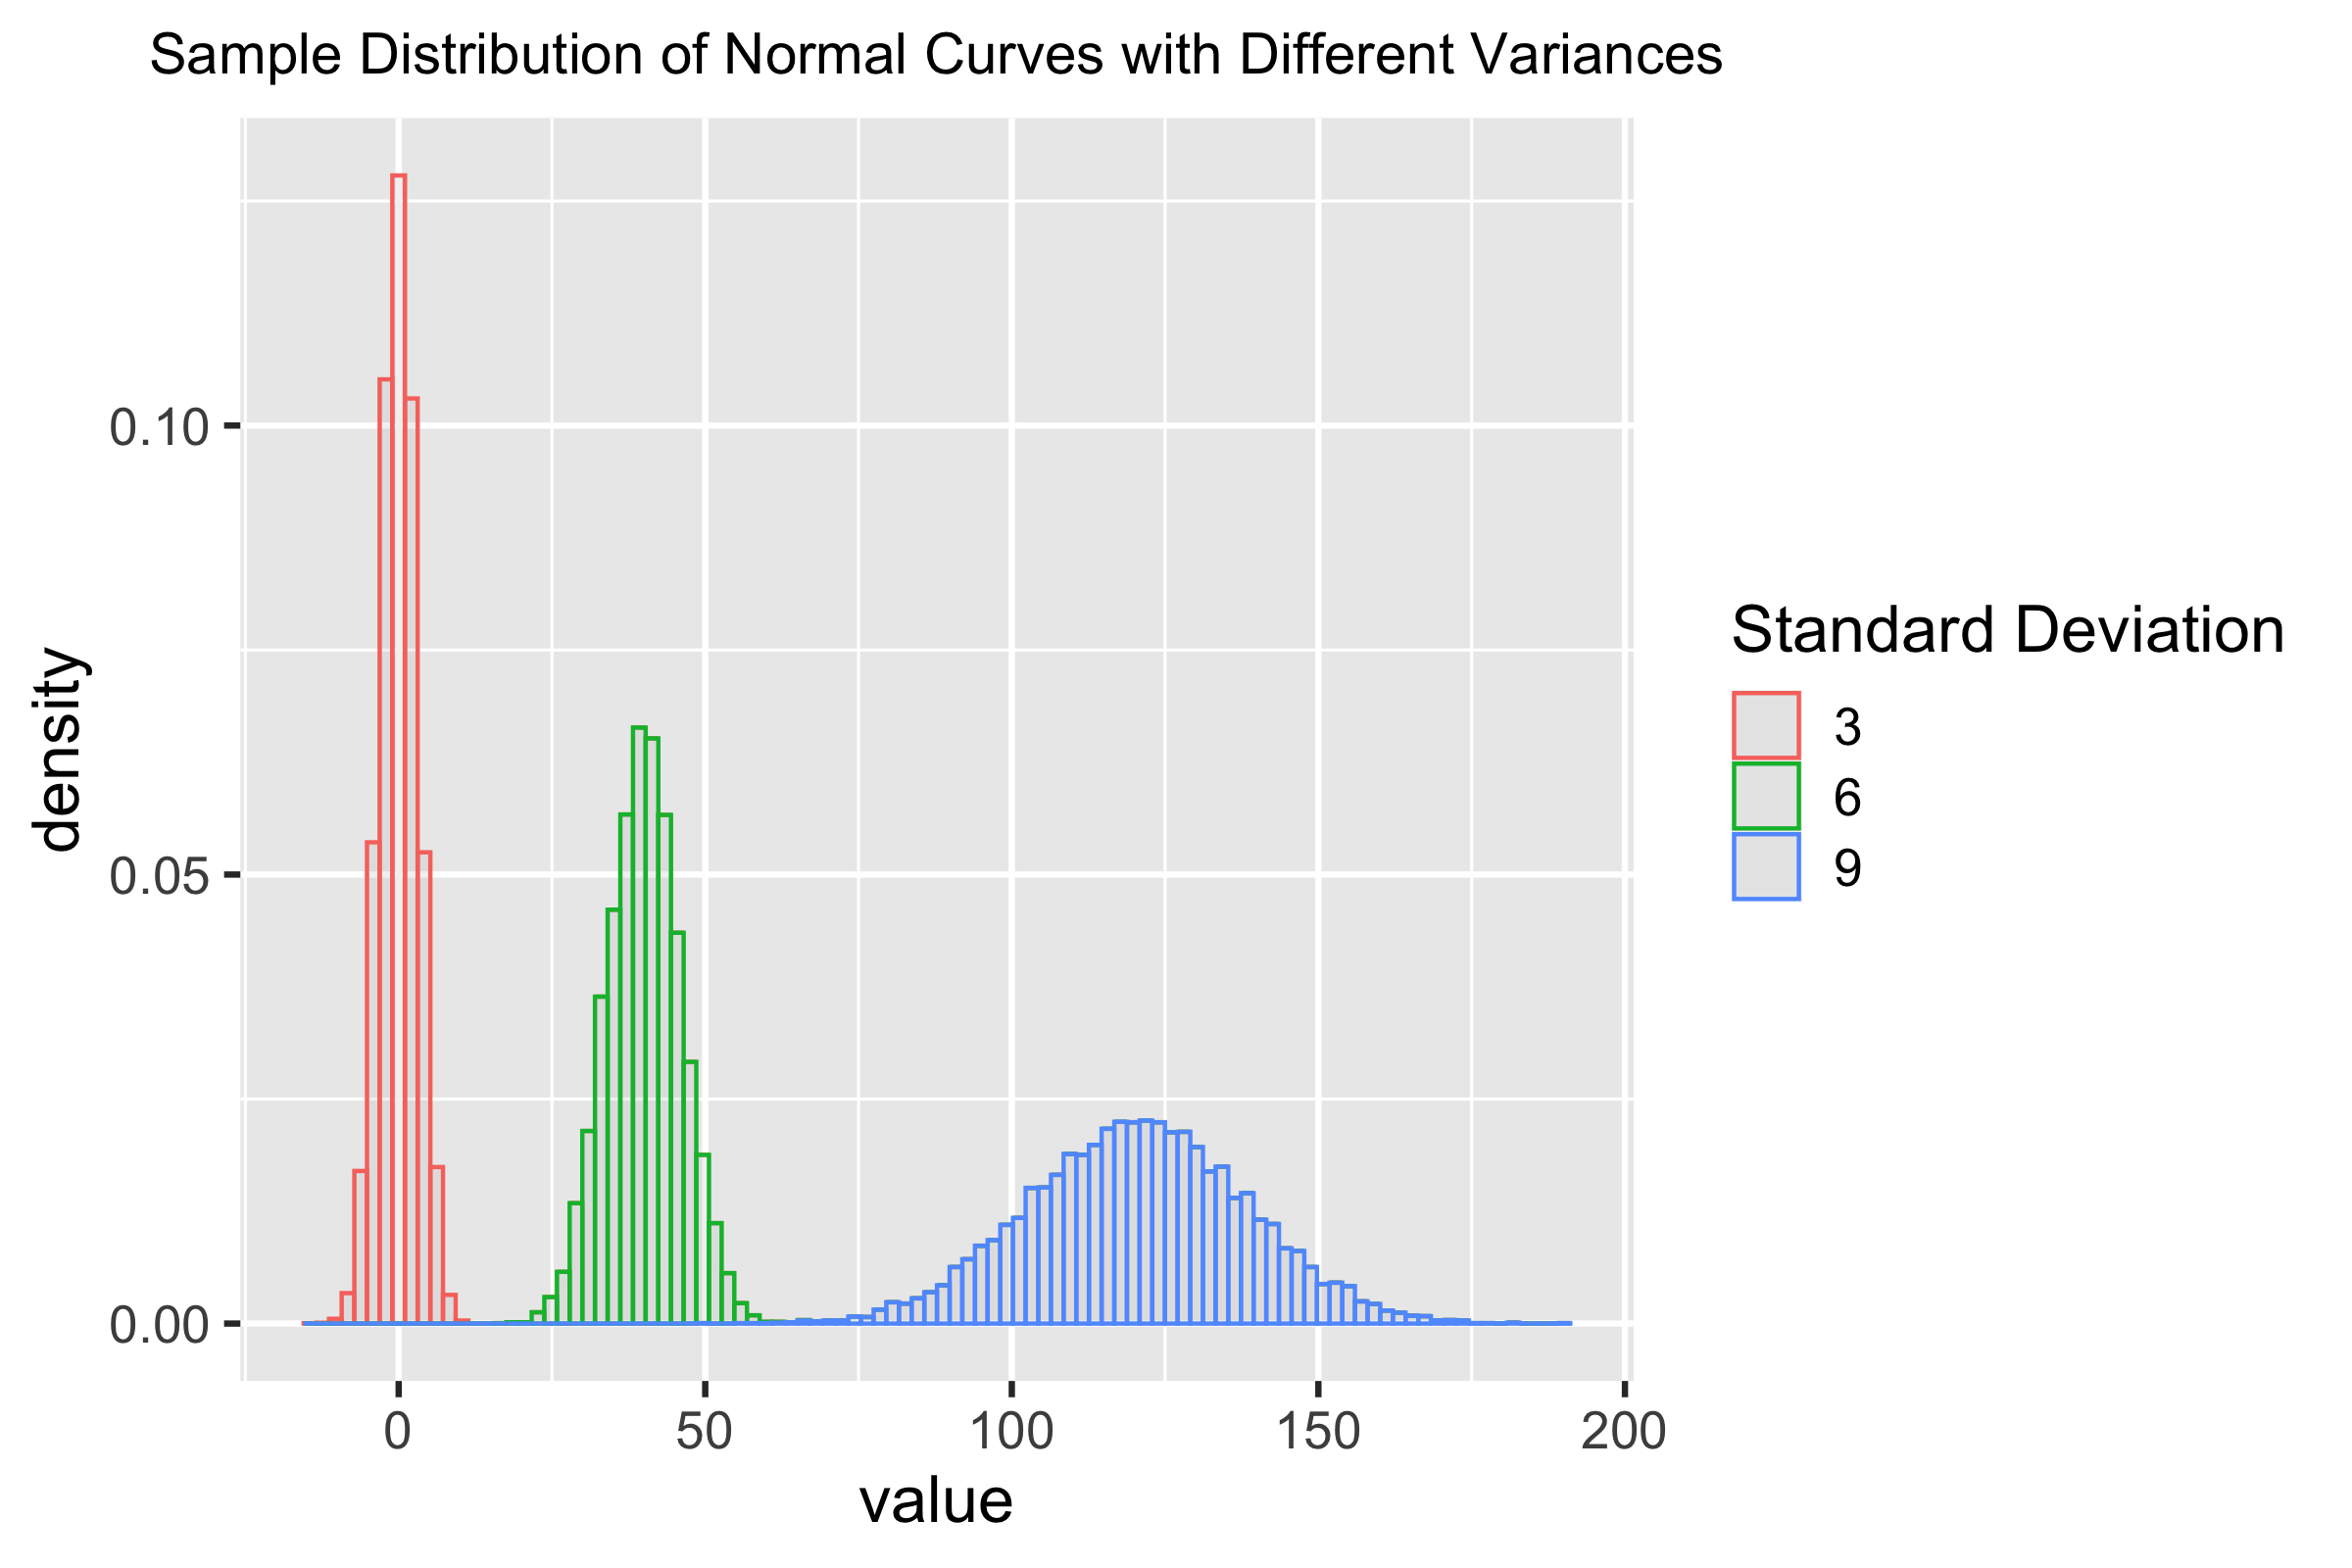
\includegraphics[width=\textwidth]{normdist_multiplevars.png}
    \end{center}
\end{frame}

\begin{frame}{68-95-99 Rule}
    \begin{center}
        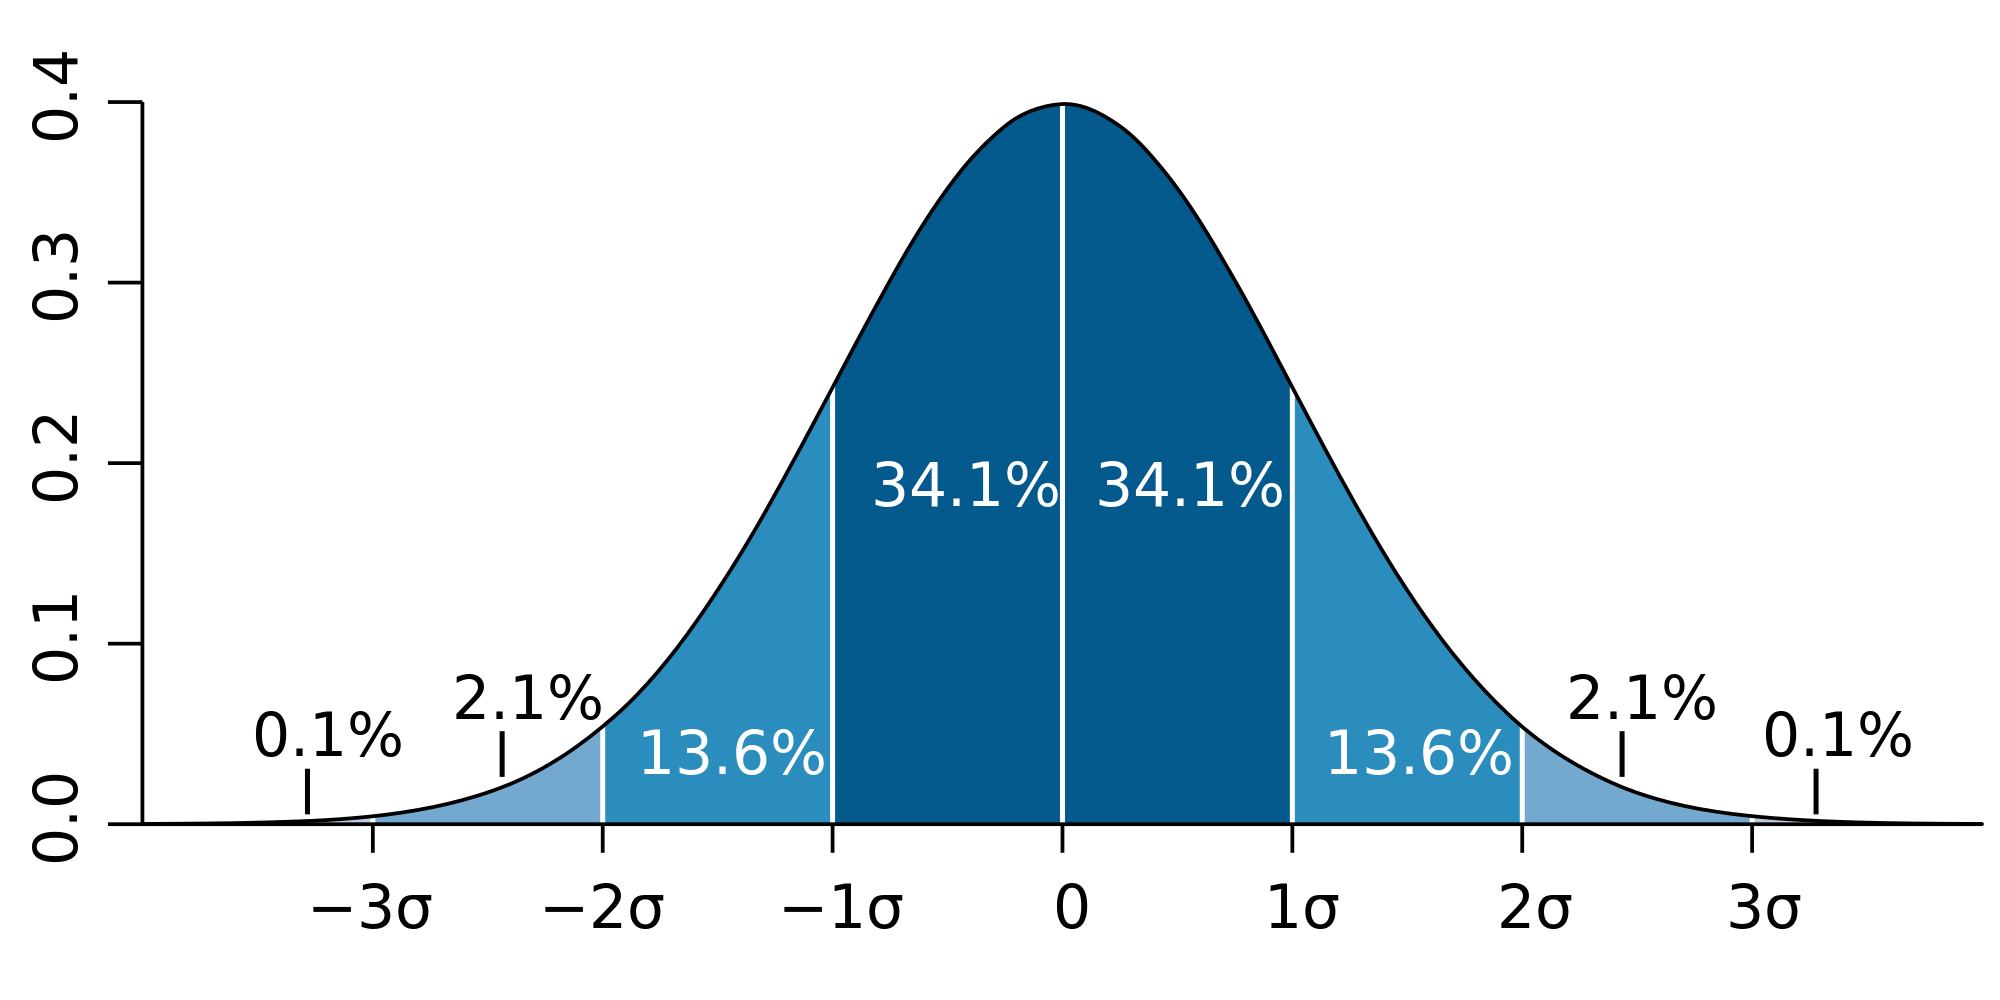
\includegraphics[width=0.8\textwidth]{stddevnorm}
    \end{center}
	
	\footnotesize{
		\begin{itemize}
			\item 68.2\% of data is within one standard deviation less than the mean and one standard deviation greater than the mean
			\item 95.4\% of data is within two standard deviations less than the mean and two standard deviations greater than the mean
			\item 99.6\% of the data is within three standard deviations less than the mean and three standard deviations greater than the mean
		\end{itemize}}
\end{frame}

\begin{frame}{Clicker Question}
	
	Suppose that the mean birthweight in the sample is 113 oz. with a standard deviation of $\sqrt{484} \approx$ 22 oz. How heavy are 95\% of babies in the sample?
	\begin{enumerate}[label=(\alph*)]
		\item 47 to 179 oz
		\item 69 to 157 oz
		\item 91 and 135 oz
		\item 111 to 120 oz
	\end{enumerate}
	
\end{frame}


\begin{frame}{Normal Distribution Notation}
	
	If X is distributed normally, we denote it the following way:
	$$X \sim N(\mu, \sigma^2)$$
	\begin{itemize} 
		\item This notation tells us everything we need to know about the normal distribution
		      \begin{itemize}
		      	\item The distribution has mean $\mu$
		      	\item The distribution has variance $\sigma^2$
		      \end{itemize}
	\end{itemize}
	
\end{frame}

\begin{frame}{Standard Normal Distribution}
	
	Standard normal distribution is a specific type of normal distribution
	\begin{itemize}
		\item If a variable X follows a normal distribution with $\mu$=0 and $\sigma^2$=1, we say that X follows the \alert{standard normal distribution}
			  
		\item Since it is so common, it is denoted as $Z \sim N(0,1)$
	\end{itemize}
	
\end{frame}

\begin{frame}{Standard Normal Distribution}
	
	\begin{itemize}
		\item The standard normal distribution is very useful
		      
		\item It is easier to find out probabilities about normal distributions if they are in the standard form
		      \begin{itemize}
		      	\item Therefore we often will \alert{standardize} any general normal distribution to be a standard normal
		      \end{itemize}
	\end{itemize}
\end{frame}


\begin{frame}{Properties of Standard Normal}
	Graph of the standard normal distribution has two important properties
	
	\begin{itemize}
		\item Symmetric
			\begin{itemize}
		      	\item $P(Z < -1) = P(Z > 1)$
			\end{itemize}
		\item Area under the curve sums to one
			\begin{itemize}
		      	\item $P(Z < 1)= 1 - P(Z > 1)$
			\end{itemize}
    \end{itemize}
    \begin{center}
        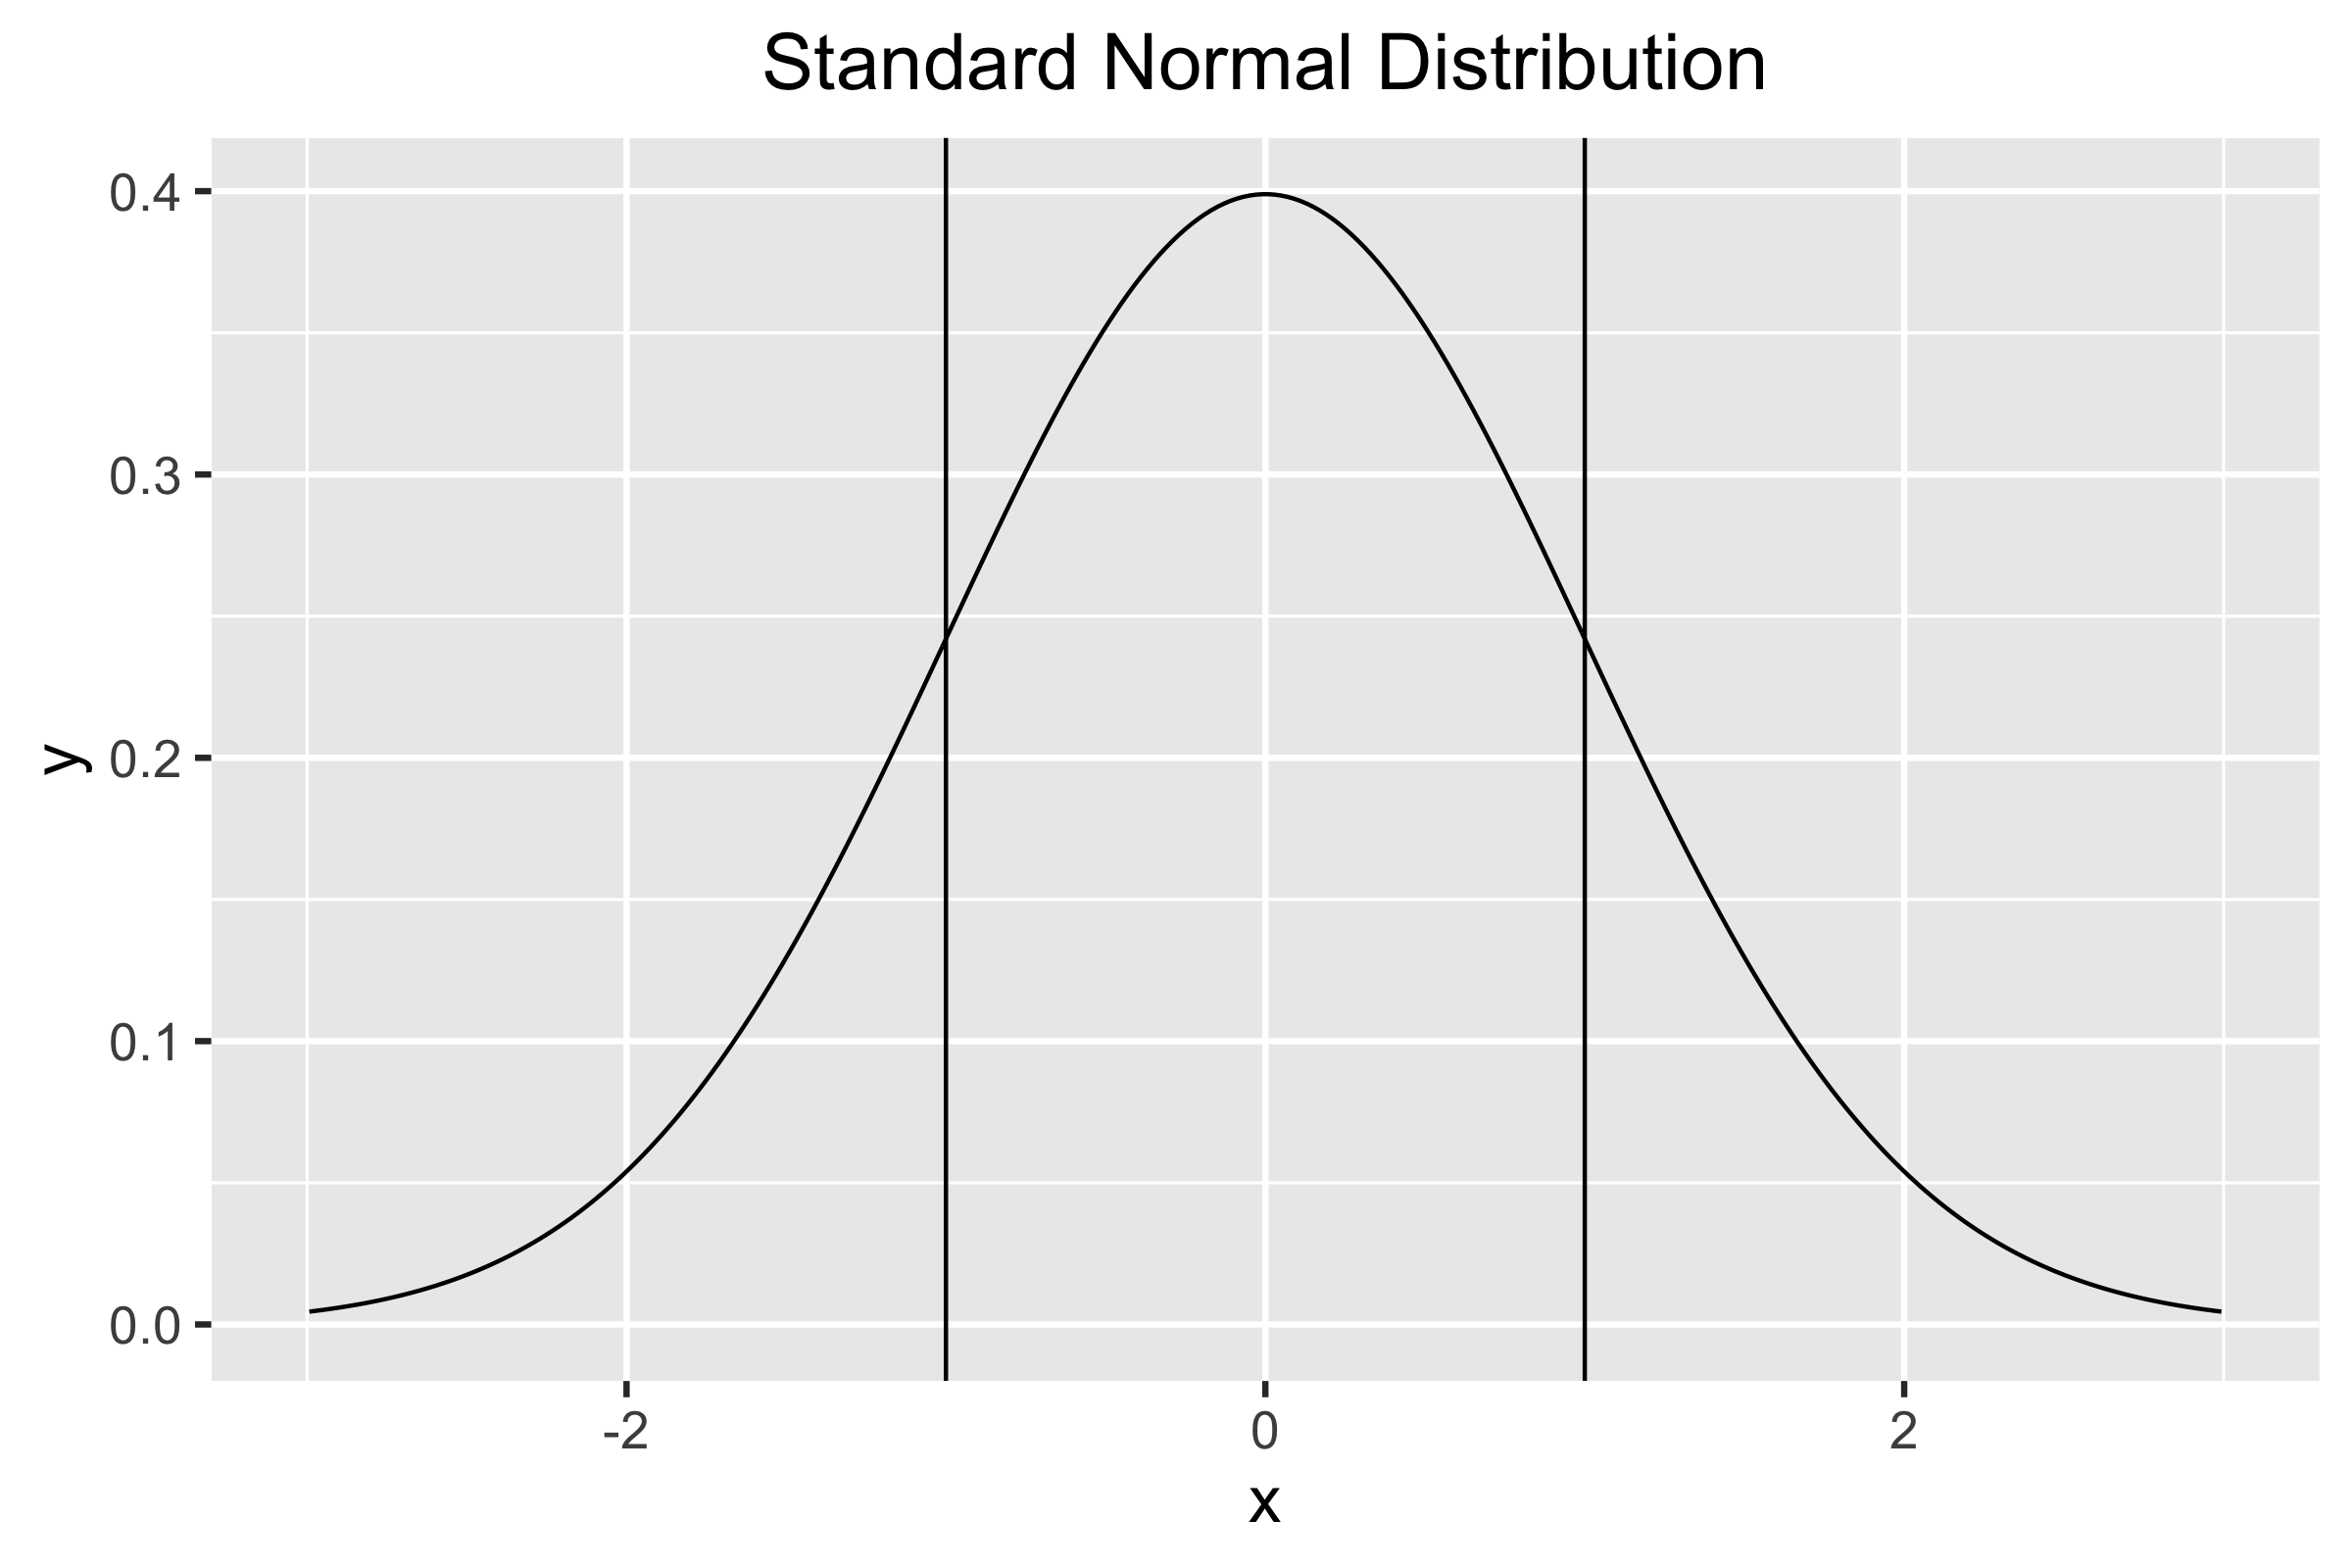
\includegraphics[width=0.6\textwidth]{stdnormal}
    \end{center}
\end{frame}

\begin{frame}{Probabilities: Cumulative Proportions}
	Suppose we want to know the likelihood of a baby being born underweight (less than 88 oz). 
	
	The data suggests $X \sim N(113,22^2).$ The probability of a baby being underweight is equal to $P(X \leq 88)$. Graphically:

	\begin{center}
		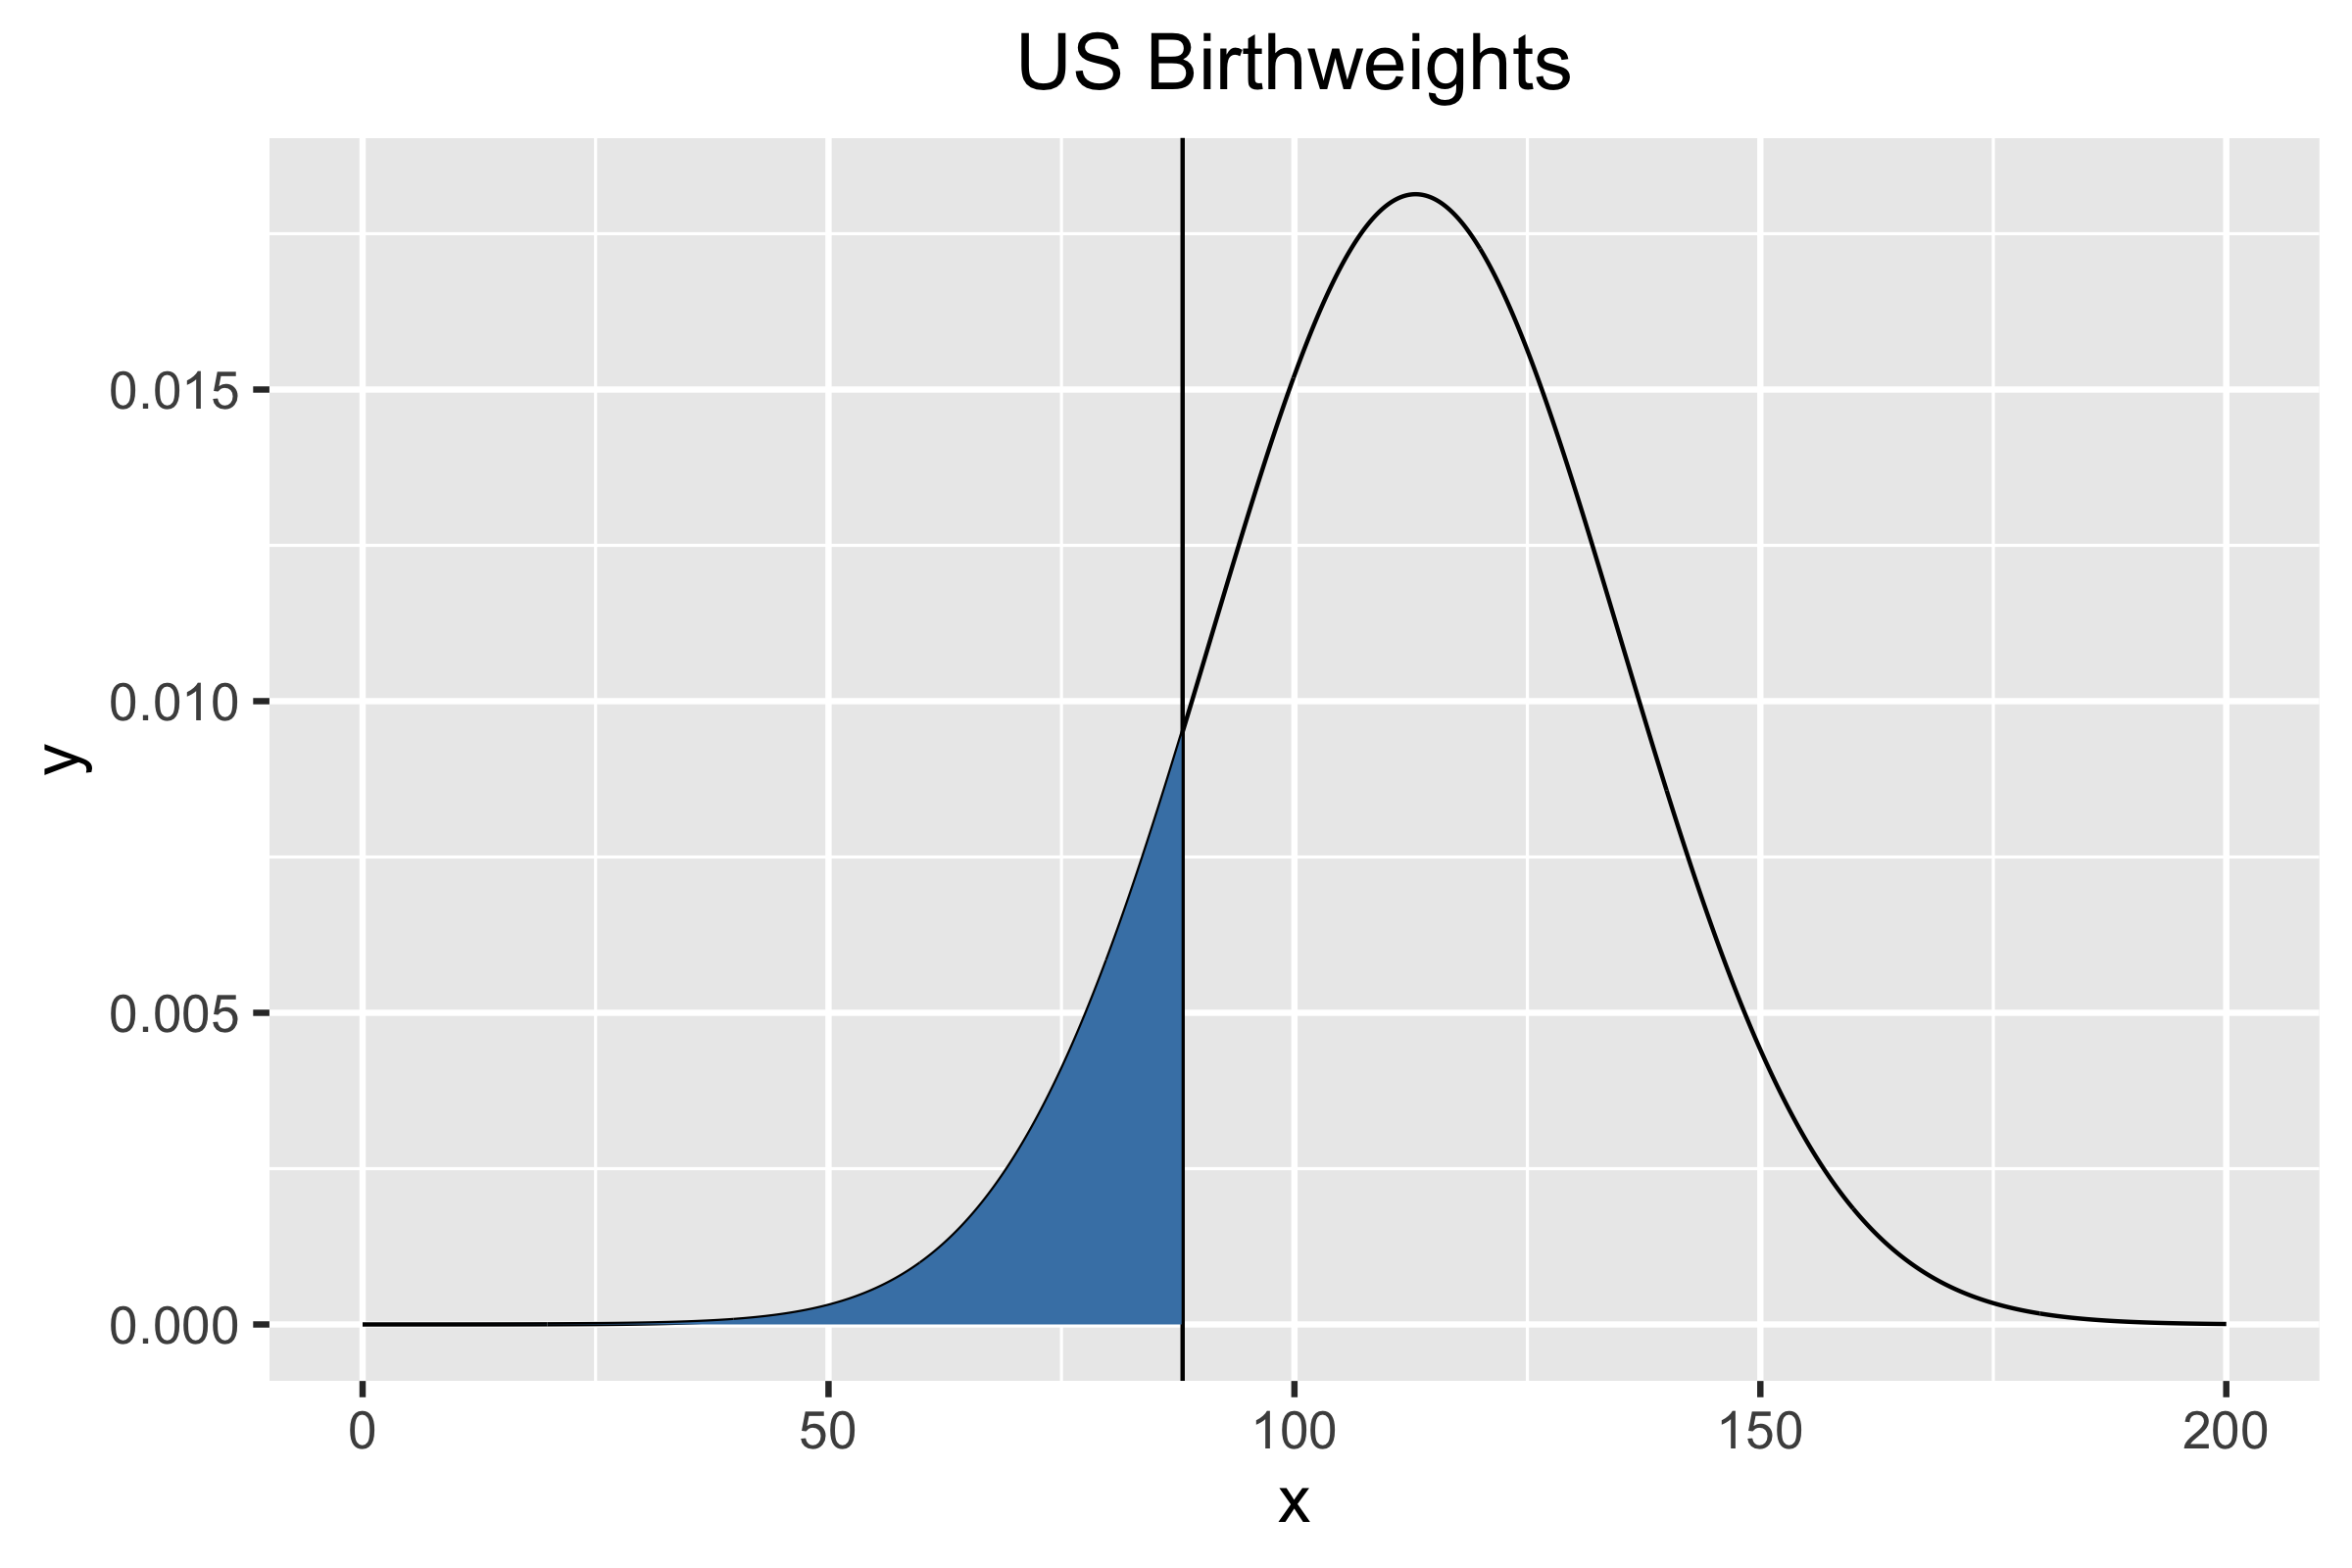
\includegraphics[width=0.75\textwidth]{normal_prob}
	\end{center}
\end{frame}



\begin{frame}{Standardization}
    
    \begin{itemize}
        \item If a variable X has any normal distribution, $X\sim N(\mu,\sigma^2)$, then the standardized variable:
        $$Z= \frac{X-\mu}{\sigma}$$
        has the standard normal distribution N(0,1)
    \end{itemize}
	
	
\end{frame}

\begin{frame}{Standardization}
	
	Z-scores are measured in standard deviations, which allows for comparison across any sample, and we don't have to worry about units.
	
	For example:
	\begin{itemize}
		\item SAT scores are $X\sim N(1500, 250^2)$
		\item ACT scores are $Y \sim N(20.8, 2.8^2)$
		\item You scored an 1860 on the SAT, your neighbor scored a 29 on the ACT. Who did better?
	\end{itemize}
	\begin{enumerate}[label=(\alph*)]
		\item You did
		\item Your neighbor
		\item You both did the same
		      
	\end{enumerate}
\end{frame} 

\begin{frame}{Standard Normal Tables}
    
    \begin{center}
        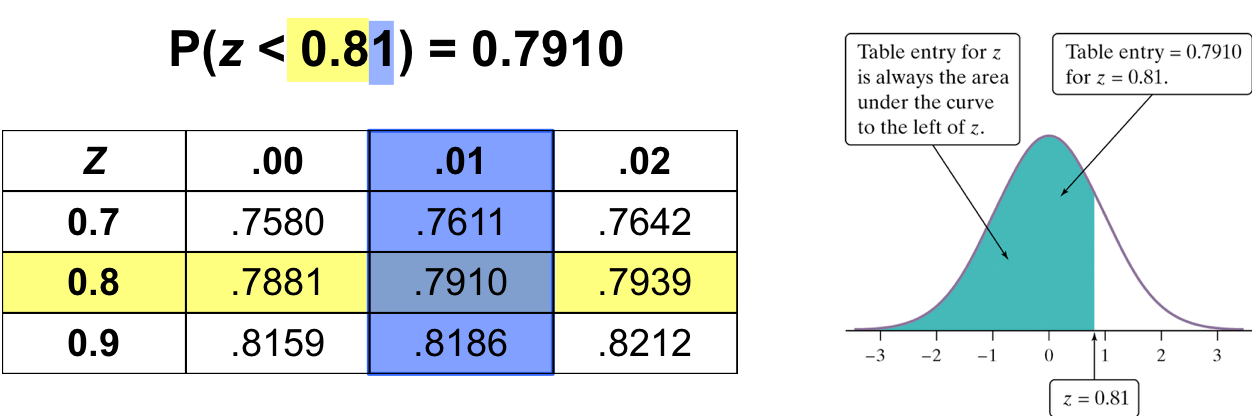
\includegraphics[width=\textwidth]{stdnormtableex}
    \end{center}

	\begin{itemize}
        \item Standard normal tables show the cumulative probability of different z-scores
		\item A table like this shows the \alert{left-tail} probabilities. 
		
		\item \textbf{Be careful!}  Some (but not many) tables display \alert{right-tail} probabilities -- areas to the right of z.
    \end{itemize}

\end{frame}

\begin{frame}{Standard Normal Table Negative}
    \begin{center}
        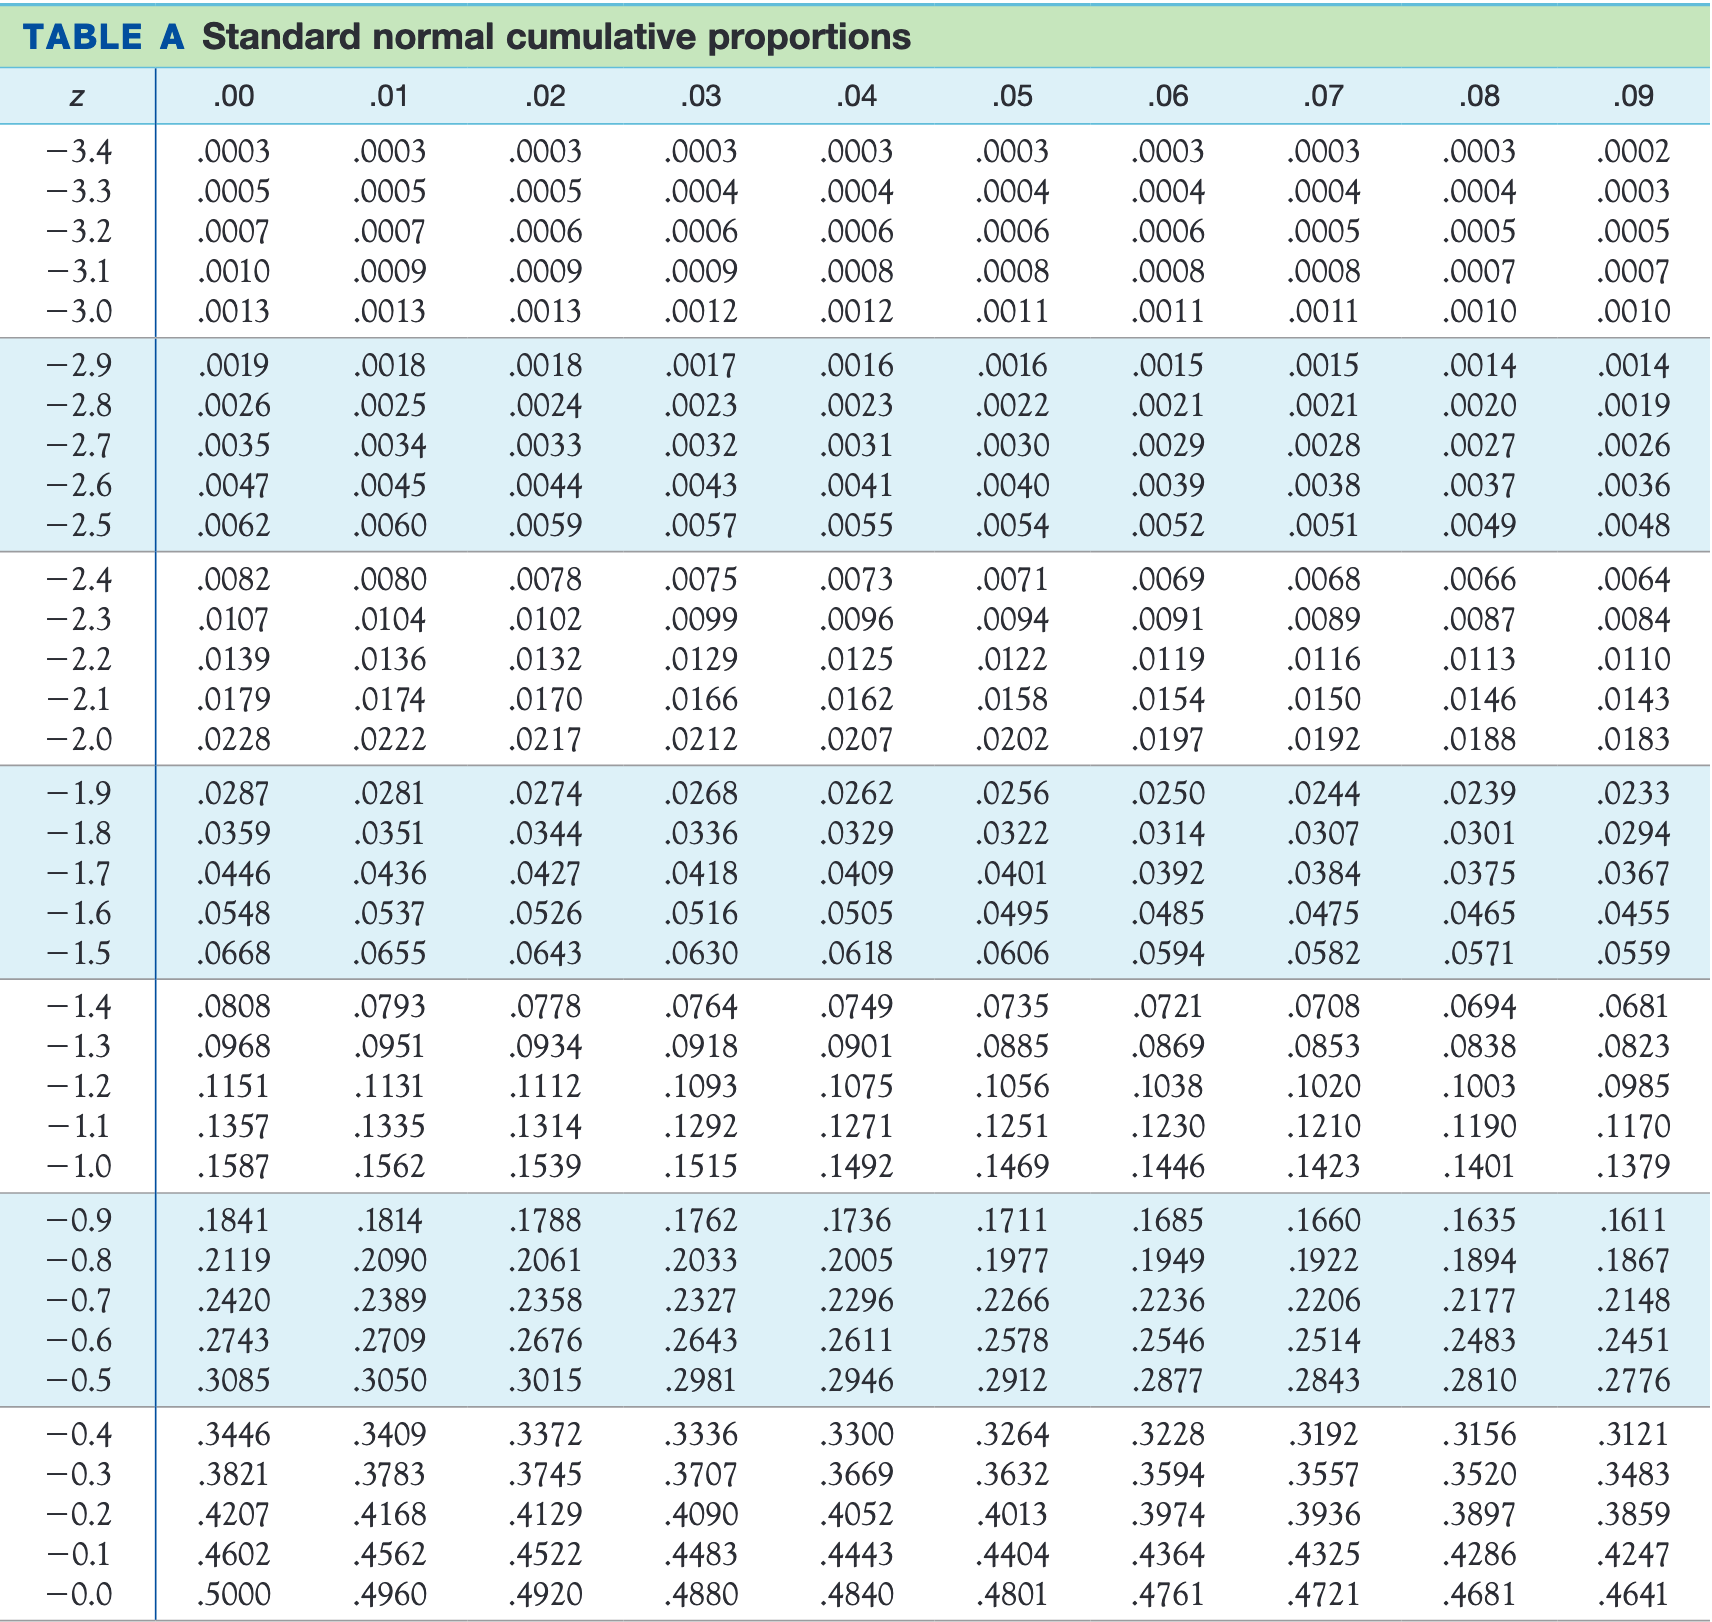
\includegraphics[width=0.8\textwidth]{z-table_neg.png}
    \end{center}
\end{frame}

\begin{frame}{Standard Normal Table Positive}
    \begin{center}
        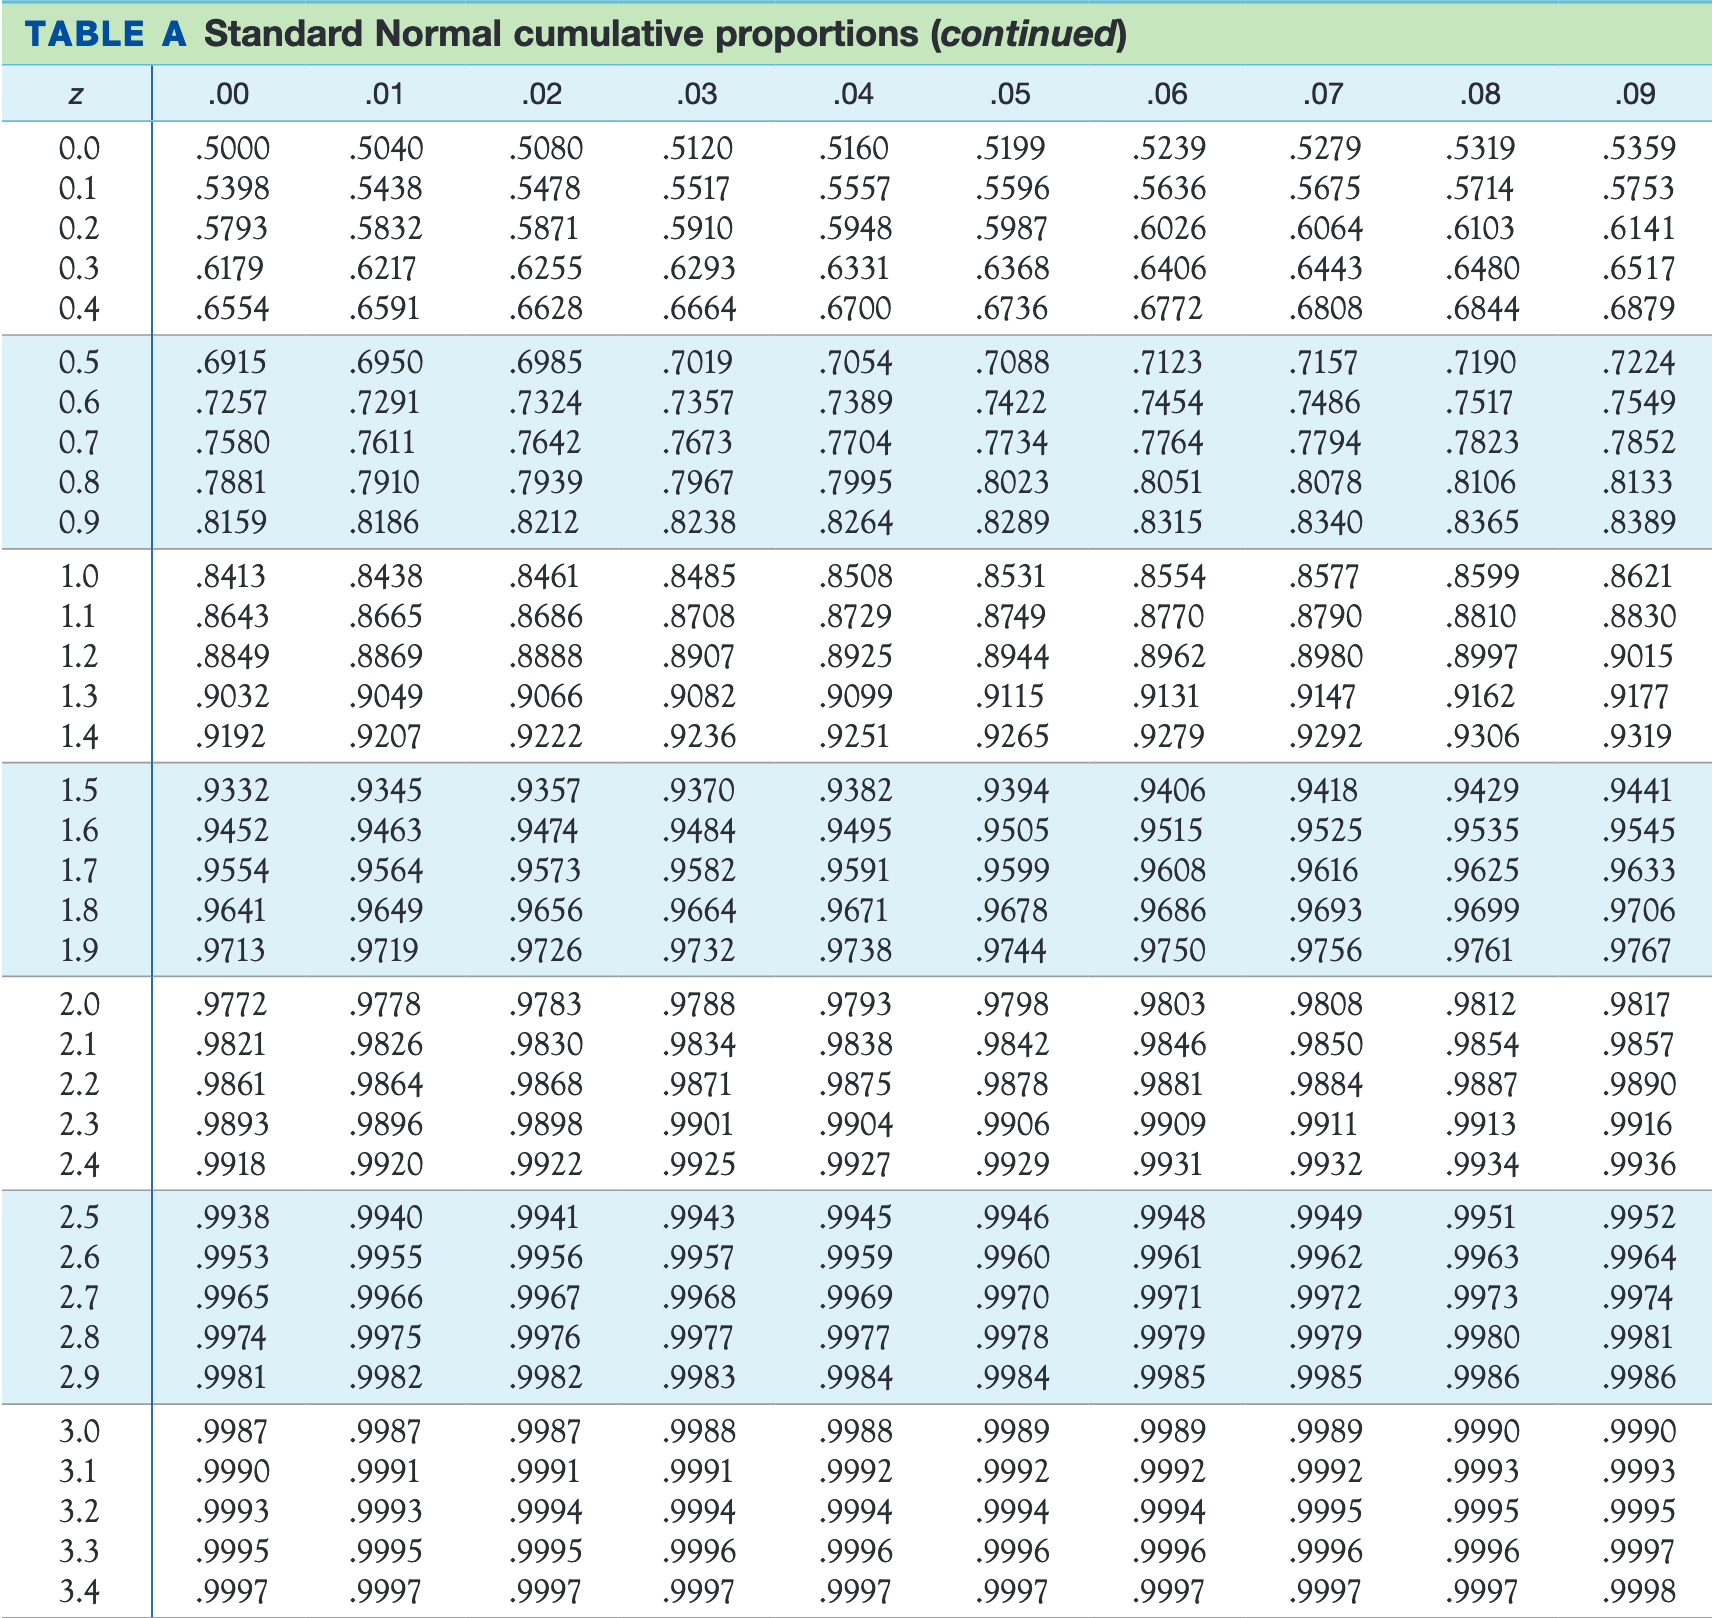
\includegraphics[width=0.8\textwidth]{z-table_pos.png}
    \end{center}
\end{frame}


\begin{frame}{Calculating Probabilities}
	How do we actually  calculate $P(X\leq88)$ \\
	(when $X\sim N(113,22^2)$)
	
	\begin{itemize}
		\item Standardize the distribution 
		      $$P(X\leq88)=P(\frac{X-\mu}{\sigma} \leq \frac{88-113}{22}) = P(Z \leq -1.14)$$
		\item Use the Z-table
		      \begin{itemize}
		      	\item May need to us properties of standard normal distribution
		      	      \begin{itemize}
		      	      	\item No negative values on table
		      	      	\item Table is either left-tail or right-tail (\alert{Z table on exam is left-tailed})
		      	      \end{itemize}
		      \end{itemize}
	\end{itemize}
\end{frame}

\begin{frame}{Using a Z-Table}
    \begin{itemize}
        \item Method 1, If you have negative values in Z-Table: 
        
        Look up Z = -1.14 in z-table

        \item Method 2, If you have only positive values in Z-Table:
        \begin{align*}
            P(Z \leq -1.14) &= P(Z \geq 1.14) \\
            &= 1-P(Z \leq 1.14) \\
            &= 1-.8729 \\ 
            &= 0.1271
        \end{align*}
    
        
    \end{itemize}
\end{frame}

\begin{frame}{Normal Example}
	
	A company chooses its new entry-level employees from a pool of recent college graduates. The cumulative GPA of the candidates is used as a tie-breaker. GPAs for the successful interviewees are normally distributed, with a mean of 3.3 and a standard deviation of 0.4. What proportion of candidates have a GPA under 3.0?
	
	\begin{enumerate}[label=(\alph*)]
		\item 0.023%
		\item 0.227
		\item 0.551
		\item 0.773
	\end{enumerate}
	
\end{frame}

\begin{frame}{Clicker Question}
	
	Consider the scenario on the previous slide, where $GPA \sim N(3.3,0.4^2)$. What percent of candidates have a $GPA$ above 3.9?
	
	\begin{enumerate}[label=(\alph*)]
		\item 2.3\%
		\item 6.7\% %%
		\item 93.3\%
		\item 97.7\%
	\end{enumerate}
	
\end{frame}

%\begin{frame}{Clicker Question -- Midterm Example}
%The average time taken for your Internet service provider to remotely resolve a trouble ticket has a Normal distribution, with a mean of 4.3 hours and a standard deviation of 3.1 hours. What percentage of tickets are resolved in less than half an hour?
%
%\begin{enumerate}[label=(\alph*)]
%\item 11.0\%
%\item 14.5\%
%\item 85.5\%
%\item 89.1\%
%\end{enumerate}
%\end{frame}

\begin{frame}{Area In Between Z-Scores}
	Suppose we want to calculate $P(-1.13 \leq Z \leq 0.3)$
	Graphically we want to calculate the following shaded area:
	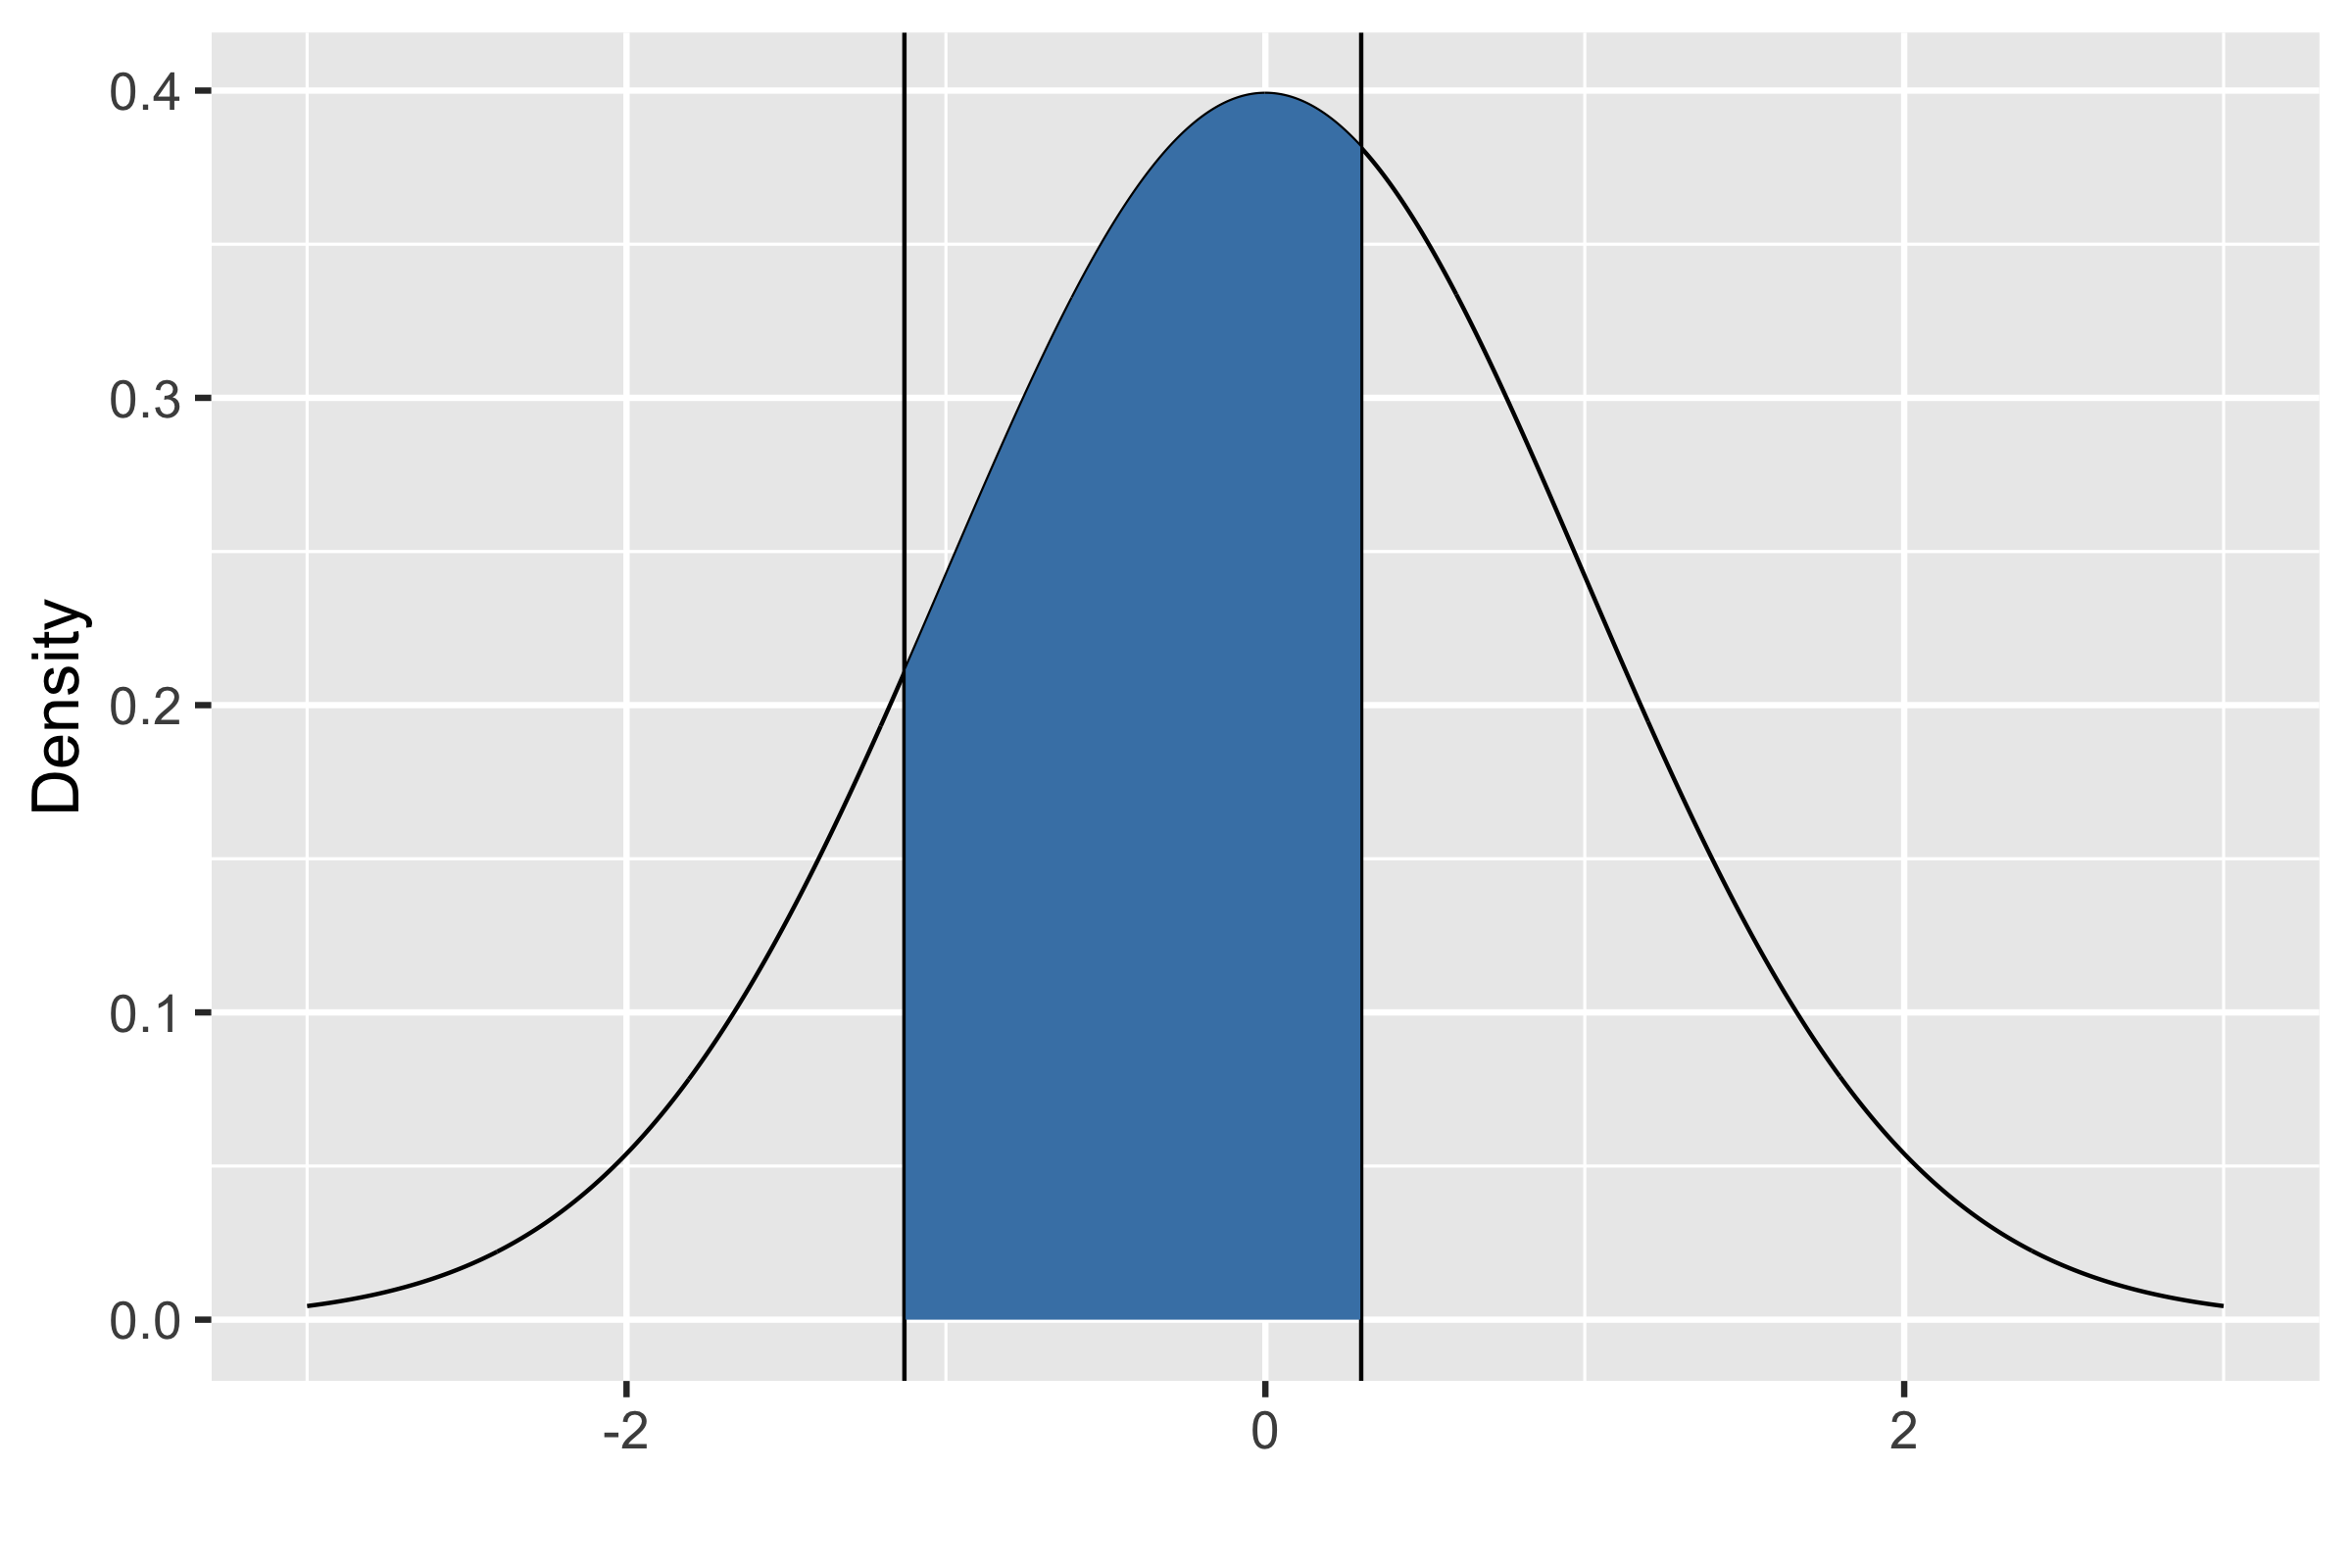
\includegraphics[width=0.8\textwidth]{areabetweenstdnorm}
\end{frame}

\begin{frame}{Area In Between Z-Scores}
	In order to calculate the area between two z-scores, 
	\[ 
		P(-1.13 \leq Z \leq 0.3) = P(Z \leq 0.3) - P(Z \leq -1.13)
	\]
	So we calculate:
	\begin{itemize}
		\item $P(Z \leq 0.3) = 0.6179$
		\item $P(Z \leq -1.13) = 0.1292$
	\end{itemize}
	
	\begin{align*}
		P(-1.13 \leq Z \leq 0.3) &= P(Z \leq 0.3) - P(Z \leq -1.13) \\ 
		&= 0.6179-0.1292 = 0.4887
	\end{align*}
\end{frame}

\begin{frame}{Clicker Question}
	A typical college freshman spends an average of $\mu=150$ minutes per day with a standard deviation of $\sigma=50$ minutes, on social media. The distribution of time on social media is known be Normal. What is the probability a college freshman spends between 2 and 3 hours on social media?
	
	\begin{enumerate}[label=(\alph*)]
		\item 0.7257
		\item 0.2743
		\item 0.4514
		\item -0.4514
	\end{enumerate}
\end{frame} 



\begin{frame}{Using probability to calculate Z-score}
	So far, we've used z-scores to calculate probabilities (values inside the table)
	
	In some cases, we will use probabilities to calculate z-scores (values outside the table)
\end{frame}

\begin{frame}[t]{Example}
	Scores on the SAT verbal test follow approximately the $N(515,109^2)$ distribution. How high must a student score in order to place in top 5\% of all students taking the SAT?
\end{frame}


\begin{frame}[t]{Example}
	
	Back to the example discussing the distribution of GPAs, where GPA  $\sim N(3.3, 0.4^2)$. If the company is interviewing 163 people, but only 121 can be hired, then what cut-off GPA should the company use?
	
\end{frame}



\begin{frame}{Clicker Question}
	Suppose that $P(Z\leq z^*) = 0.025$. Using a standard normal table, find $z^*$
	
	\begin{enumerate}[label=(\alph*)]
		\item 0.5478
		\item -0.5478
		\item 1.96
		\item -1.96
	\end{enumerate}
\end{frame}

\begin{frame}[t]{Review of Normal Distribution}
	Consider men's height to be distributed normally with a mean of 5.9 feet and a standard deviation or 0.4 feet.
	Calculate the following:
	\begin{itemize}
		\item $P(X>6.5)$
		      
		\item $P(X>5)$
		      
		\item What is the top 10\% of men's height?
		      
		\item What is the bottom 20\% of men's height?
	\end{itemize}
\end{frame}

\begin{frame}

\end{frame}




\end{document}